%%%%%%%% ICML 2025 SUBMISSION — Safe Learning to Defer for Insurance Fraud Detection %%%%%%%%

\documentclass{article}

\usepackage{microtype}
\usepackage{graphicx}
\usepackage{subfigure}
\usepackage{booktabs}
\usepackage{hyperref}
\usepackage{float}
\newcommand{\theHalgorithm}{\arabic{algorithm}}

\usepackage[accepted]{icml2025}

\usepackage{amsmath}
\usepackage{amssymb}
\usepackage{mathtools}
\usepackage{amsthm}
\usepackage[capitalize,noabbrev]{cleveref}

\usepackage{algorithm}
\usepackage{algorithmic}
\usepackage{enumitem}

%%%%%%%%%%%%%%%%%%%%%%%%%%%%%%%%
% THEOREMS
%%%%%%%%%%%%%%%%%%%%%%%%%%%%%%%%
\theoremstyle{plain}
\newtheorem{theorem}{Theorem}[section]
\newtheorem{proposition}{Proposition}[section]
\newtheorem{lemma}{Lemma}[section]
\newtheorem{corollary}{Corollary}[section]
\theoremstyle{definition}
\newtheorem{definition}{Definition}[section]
\newtheorem{assumption}{Assumption}[section]
\theoremstyle{remark}
\newtheorem{remark}{Remark}[section]

%%%%%%%%%%%%%%%%%%%%%%%%%%%%%%%%
% CUSTOM COMMANDS
%%%%%%%%%%%%%%%%%%%%%%%%%%%%%%%%
\newcommand{\cvar}{\mathrm{CVaR}}
\newcommand{\var}{\mathrm{VaR}}
\newcommand{\deferop}{\textsc{Defer}}
\newcommand{\xx}{\mathbf{x}}
\newcommand{\RR}{\mathbb{R}}
\newcommand{\EE}{\mathbb{E}}
\newcommand{\PP}{\mathbb{P}}
\DeclareMathOperator*{\argmin}{arg\,min}
\DeclareMathOperator*{\argmax}{arg\,max}

\icmltitlerunning{Safe Learning to Defer for Insurance Fraud Detection}

\begin{document}

\twocolumn[
\icmltitle{Safe Learning to Defer for Insurance Fraud Detection:\\
           A Risk-Sensitive Framework}

\icmlsetsymbol{equal}{*}

\begin{icmlauthorlist}
\icmlauthor{Samuel Zhang}{dept}
\icmlauthor{Miltiades Georgantzis}{dept}
\icmlauthor{Sulieman Ibsais}{dept}
\end{icmlauthorlist}

\icmlaffiliation{dept}{Department of EEE, Imperial College London, London, United Kingdom}

\icmlcorrespondingauthor{Samuel Zhang}{sjz25@ic.ac.uk}

\icmlkeywords{Learning to Defer, Fraud Detection, CVaR, Bayesian Uncertainty, Risk-Sensitive ML}

\vskip 0.3in
]

\printAffiliationsAndNotice{}

\begin{abstract}
Automated fraud detection systems have to make a call on every case, even when the model is not very sure. We introduce \textbf{Safe-L2D-Fraud}, a framework for insurance fraud detection that combines learning to defer (L2D) with Conditional Value-at-Risk (CVaR)-based threshold selection. A pre-trained classifier first generates predictions and uncertainty estimates. Then a deferral policy sends the most unclear claims to human investigators, while also penalising errors in the worst-$\delta$ fraction of cases the system keeps. The deferral decision brings together two signals, Bayesian posterior entropy and calibrated classifier confidence, and uses domain-informed feature selection based on a directed acyclic graph. In a proof-of-concept evaluation on a 1{,}000-claim insurance dataset, Safe-L2D-Fraud reaches 89.5\% system accuracy (95\% CI: [85.0\%, 93.5\%]) at 64\% coverage, improving over standalone XGBoost by 7.5 percentage points, though confidence intervals between methods overlap. We evaluate the framework using bootstrap confidence intervals and cross-validation, and provide a detailed assessment of limitations including small sample size, distribution shift, and adversarial non-stationarity.
\end{abstract}

\section{Introduction}
\label{sec:intro}

Insurance fraud is estimated to cost the U.S.\ economy \$308.6 billion a year, with fraudulent claims making up 5--10\% of all property and casualty claims \citep{coalition2022fraud}. Supervised classifiers such as gradient boosted trees, logistic regression, and neural networks have become standard tools for detecting fraud \citep{phua2010comprehensive}. But these models still have to make a yes-or-no decision on every claim, even when they are highly uncertain.

The \textit{learning to defer} (L2D) paradigm tackles this problem by giving the classifier a deferral option, so uncertain cases can be passed to a human expert instead \citep{madras2018predict, mozannar2020consistent}. This is especially well-suited to fraud detection. The costs of false negatives, where fraud is missed, and false positives, where legitimate claims are wrongly denied, are very different, and human investigators can add valuable domain knowledge that the model does not have.

Standard L2D methods, however, optimise \textit{expected} loss, which means they treat all retained errors the same way. In fraud detection, the \textit{distribution} of those errors also matters. A small number of high-value missed claims can account for a large share of the total loss. So deferral should focus not only on uncertainty, but also on the claims that contribute most to \textit{tail risk}.

We make the following contributions:
\begin{enumerate}
    \item We propose \textbf{Safe-L2D-Fraud}, a two-stage framework that separates classifier training from deferral optimisation, and selects the deferral threshold using a CVaR-penalised objective (\Cref{def:cvar_l2d}).
    \item We combine \textbf{Bayesian posterior entropy} with calibrated classifier confidence for deferral, using a domain-informed DAG to limit uncertainty estimation to structurally plausible features.
    \item We present a \textbf{proof-of-concept evaluation} on a small benchmark dataset that demonstrates the framework's mechanics, including cost-sensitive analysis and ablations, accompanied by a frank assessment of \textbf{limitations} including small sample size, distribution shift, and adversarial non-stationarity. We view the primary contribution as the framework design rather than the specific empirical numbers.
\end{enumerate}
\section{Background}
\label{sec:background}

\subsection{Learning to Defer}
\label{sec:bg_l2d}

The learning-to-defer framework jointly trains a classifier $h: \mathcal{X} \to \mathcal{Y}$ and a rejector $r: \mathcal{X} \to \{0, 1\}$ that decides whether each input should be deferred to a human expert $M$ \citep{madras2018predict}. \citet{mozannar2020consistent} showed that this setup can be reduced to a $(K{+}1)$-class classification problem. For binary classification ($K=2$), the system outputs $g: \mathcal{X} \to \RR^3$ with components for class~0 (predict not-fraud), class~1 (predict fraud), and $\perp$ (defer). The surrogate cross-entropy loss is:
\begin{equation}
    \tilde{L}_{\text{CE}}(g, \xx, y, m) = -\sum_{j \in \{0,1,\perp\}} c_j \log \frac{e^{g_j(\xx)}}{\sum_k e^{g_k(\xx)}},
    \label{eq:mozannar_loss}
\end{equation}
where the cost targets encode misclassification penalties: $c_0 = \mathbf{1}[y{=}1]$ penalises predicting class~0 (not-fraud) when the true label is fraud, $c_1 = \mathbf{1}[y{=}0]$ penalises predicting class~1 (fraud) when the claim is legitimate, and $c_\perp = \ell_{\text{exp}}(\xx, y, M) = \PP(M(\xx) \neq y)$ is the expert's expected 0-1 loss on the deferred instance. This means the correct action, the one with zero misclassification cost, gets zero weight, which encourages the model to assign it high probability. Minimising this surrogate gives a Bayes-consistent deferral policy \citep{mozannar2020consistent}.

\subsection{Conditional Value-at-Risk}
\label{sec:bg_cvar}

For a random loss $Z$, the Conditional Value-at-Risk at tail level $\delta \in (0,1]$ is:
\begin{equation}
    \cvar_\delta(Z) = \frac{1}{\delta} \EE\bigl[Z \cdot \mathbf{1}\{Z \geq \var_\delta(Z)\}\bigr],
    \label{eq:cvar}
\end{equation}
where $\var_\delta(Z) = \inf\{z : \PP(Z \leq z) \geq 1 - \delta\}$. CVaR is coherent, sub-additive, and convex \citep{rockafellar2000optimization}, and it has been used to control catastrophic tail risks in risk-sensitive RL \citep{tamar2015optimizing} and safety-critical offline RL \citep{killian2023risk}.

\subsection{Bayesian Uncertainty for Classification}
\label{sec:bg_bayes}

Given class-conditional densities $p(\xx | y{=}1)$ and $p(\xx | y{=}0)$ estimated via KDE, the posterior fraud probability after observing features $(x_1, \ldots, x_F)$ is obtained through sequential Bayesian updating:
\begin{equation}
    \pi_k = \frac{\pi_{k-1} \cdot p(x_k | y{=}1)}{\pi_{k-1} \cdot p(x_k | y{=}1) + (1 - \pi_{k-1}) \cdot p(x_k | y{=}0)},
    \label{eq:bayes_update}
\end{equation}
starting from the prior $\pi_0 = \PP(y{=}1)$. This assumes conditional independence given the class label (Assumption~A1, \Cref{sec:exp_setup}). The binary entropy $H(\pi) = -\pi \log_2 \pi - (1{-}\pi) \log_2 (1{-}\pi)$ measures predictive uncertainty.
\section{Problem Formulation}
\label{sec:formulation}

\subsection{Fraud Detection as Learning to Defer}
\label{sec:fraud_l2d}

We model insurance fraud detection as a learning-to-defer problem. Each claim $\xx \in \mathcal{X} \subseteq \RR^d$ has a binary label $y \in \{0, 1\}$ (legitimate or fraudulent). The system must choose one of three actions: $a \in \{\text{clear}, \text{flag}, \deferop\}$. When the system defers, a human fraud investigator $M$ examines the claim with accuracy parameterised by $\alpha \in (0, 1]$.

The \textit{system-level} prediction is:
\begin{equation}
    \hat{y}_{\text{sys}}(\xx) = \begin{cases}
        h(\xx) & \text{if } r(\xx) = 0 \quad (\text{classifier decides}), \\
        M(\xx) & \text{if } r(\xx) = 1 \quad (\text{investigator decides}).
    \end{cases}
\end{equation}
The \textit{coverage} is the fraction of claims decided by the classifier: $\text{Coverage} = 1 - \frac{1}{N}\sum_{i} r(\xx_i)$.

\subsection{Two-Stage Risk-Sensitive Deferral}
\label{sec:risk_objective}

Since the base classifier $h$ is typically pre-trained or provided by a third party, we decouple classifier training from deferral optimisation: Stage~1 trains $h$ via standard supervised learning, and Stage~2 selects the rejector $r$ by optimising a CVaR-penalised objective over the deferral threshold. Formally:

\begin{definition}[CVaR-Guided Deferral Objective]
\label{def:cvar_l2d}
Given a fixed classifier $h$, risk level $\delta \in (0,1]$, and trade-off weight $\lambda > 0$, the deferral threshold $\tau$ is selected by:
\begin{equation}
\begin{aligned}
\tau^*
&= \argmax_{\tau} \;
\underbrace{\mathrm{Acc}_{\mathrm{sys}}(h, r_\tau)}_{\text{system accuracy}} \\
&\quad - \lambda \underbrace{\cvar_\delta\bigl[\ell(\xx, y, h(\xx)) \cdot \mathbf{1}\{r_\tau(\xx) = 0\}\bigr]}_{\text{tail risk on retained claims}}
\end{aligned}
\label{eq:cvar_l2d}
\end{equation}

where $r_\tau(\xx) = \mathbf{1}[U(\xx) > \tau]$ is a threshold rejector based on an uncertainty signal $U(\xx)$ (defined in \Cref{sec:method_bayes}), and $\ell(\xx, y, h(\xx)) = \mathbf{1}[h(\xx) \neq y]$ is the 0-1 loss on non-deferred instances.
\end{definition}

The first term rewards effective deferral of hard cases; the second penalises configurations where retained predictions carry high worst-case error. The CVaR term admits the Rockafellar--Uryasev dual \citep{rockafellar2000optimization}:
\begin{equation}
    \cvar_\delta[Z] = \inf_{\eta \in \RR} \left\{ \eta + \frac{1}{\delta}\EE\bigl[(Z - \eta)^+\bigr] \right\},
    \label{eq:cvar_dual}
\end{equation}
which is convex in $\eta$. Although the one-dimensional threshold sweep in \Cref{eq:cvar_l2d} does not directly exploit this convexity, the coherence and smoothness of CVaR make the objective well-behaved compared to, e.g., VaR.

\begin{proposition}[Tail-Risk Reduction via Deferral]
\label{prop:cvar_bound}
Let $r$ be any rejector that defers at least one sample. Denote $\mathcal{S}_r = \{i : r(\xx_i) = 0\}$ the retained set. If every deferred sample has loss $\ell_i \geq \var_\delta(\ell)$ (i.e., deferral targets the upper tail), then:
\begin{equation}
    \cvar_\delta\bigl[\ell_i \mid i \in \mathcal{S}_r\bigr] \leq \cvar_\delta\bigl[\ell_i\bigr].
\end{equation}
\end{proposition}
The proof is given in \Cref{app:math}. For 0-1 loss, the condition simplifies: since $\ell_i \in \{0,1\}$, the proposition requires that deferred samples include a sufficient proportion of misclassified instances. We verify this empirically in our experiments, the Spearman rank correlation between posterior entropy $H(\pi_F)$ and the 0-1 loss is $\rho > 0.3$ ($p < 0.001$), confirming that the uncertainty signal preferentially identifies misclassified claims (\Cref{sec:exp_results}).

\subsection{Connection to Constrained Optimisation}
\label{sec:cmdp}

The deferral objective in \Cref{eq:cvar_l2d} can be viewed as the Lagrangian relaxation of a constrained problem. Define:
\begin{equation}
\begin{aligned}
\max_{r} \;& \mathrm{Acc}_{\mathrm{sys}}(h, r) \\
\text{s.t.} \;& \cvar_\delta\bigl[\ell(\xx, y, h(\xx)) \cdot \mathbf{1}\{r(\xx) = 0\}\bigr] \leq \epsilon
\end{aligned}
\label{eq:cmdp}
\end{equation}

Under Slater's condition (which holds when there exists a feasible $r$ achieving $\cvar_\delta < \epsilon$, e.g., by deferring all claims), strong duality gives $\max_r \min_{\lambda \geq 0} \{\mathrm{Acc}_{\mathrm{sys}} + \lambda(\epsilon - \cvar_\delta)\} = \min_{\lambda \geq 0} \max_r \{\mathrm{Acc}_{\mathrm{sys}} + \lambda(\epsilon - \cvar_\delta)\}$, and the optimal $\lambda^*$ recovers the constraint boundary. Thus, \Cref{eq:cvar_l2d} with a specific $\lambda$ corresponds to a particular risk tolerance $\epsilon$, connecting our framework to constrained optimisation \citep{altman1999constrained}. In the sequential setting where claims arrive over time and investigator capacity is finite, this extends to a constrained MDP, motivating online deferral with budget constraints as future work.

\section{The Safe-L2D-Fraud Framework}
\label{sec:method}

This section details the four components of Safe-L2D-Fraud (\Cref{fig:system}): Bayesian uncertainty quantification (\Cref{sec:method_bayes}), combined deferral rule (\Cref{sec:method_cvar}), domain-informed feature selection (\Cref{sec:method_causal}), and off-policy evaluation (\Cref{sec:method_ope}).

\begin{figure}[H]
    \centering
    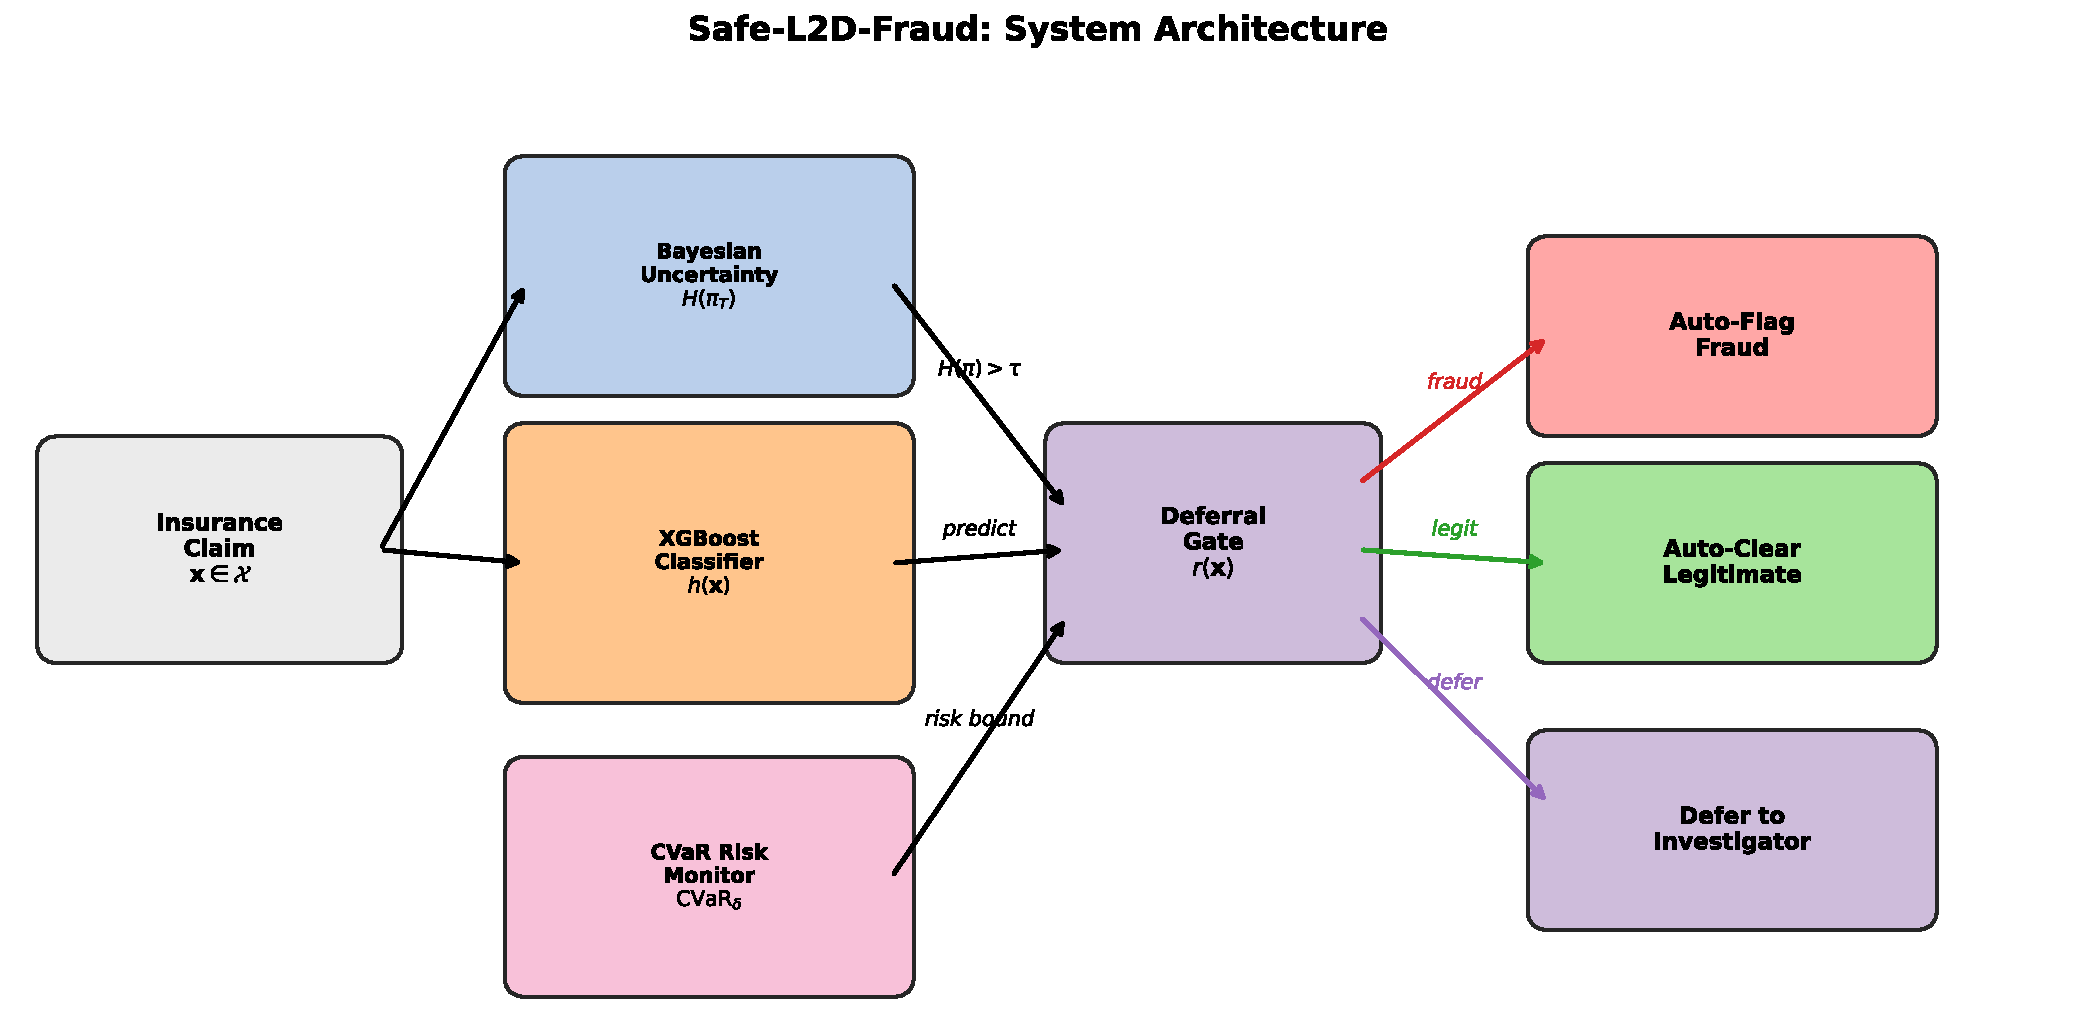
\includegraphics[width=\columnwidth]{figures/l2d_system_diagram.pdf}
    \caption{Safe-L2D-Fraud architecture. Claims flow through a Bayesian uncertainty module and XGBoost classifier. A CVaR-guided deferral gate routes uncertain claims to a human investigator, controlling tail risk on retained predictions.}
    \label{fig:system}
\end{figure}

\subsection{Bayesian Uncertainty Quantification}
\label{sec:method_bayes}

For each claim $\xx$, we estimate class-conditional densities $\hat{p}(x_k | y{=}1)$ and $\hat{p}(x_k | y{=}0)$ using Gaussian KDE on the training set, restricting to features validated by the domain-informed DAG (\Cref{sec:method_causal}). The posterior fraud probability $\pi_F$ is obtained via the sequential update in \Cref{eq:bayes_update}.

The entropy-based deferral signal is:
\begin{equation}
\begin{aligned}
U_{\text{Bayes}}(\xx)
&= H(\pi_F) \\
&= -\pi_F \log_2 \pi_F - (1{-}\pi_F)\log_2(1{-}\pi_F)
\end{aligned}
\label{eq:entropy_defer}
\end{equation}
This is maximised at $\pi_F = 0.5$ (maximum ambiguity) and decreases as $\pi_F$ moves toward 0 or 1. Claims with $U_{\text{Bayes}}(\xx) > \tau$ are candidates for deferral. \Cref{fig:class_cond} shows substantial class-conditional overlap in claim amount and policy age---the ambiguous region where deferral is most valuable.

\begin{figure}[H]
    \centering
    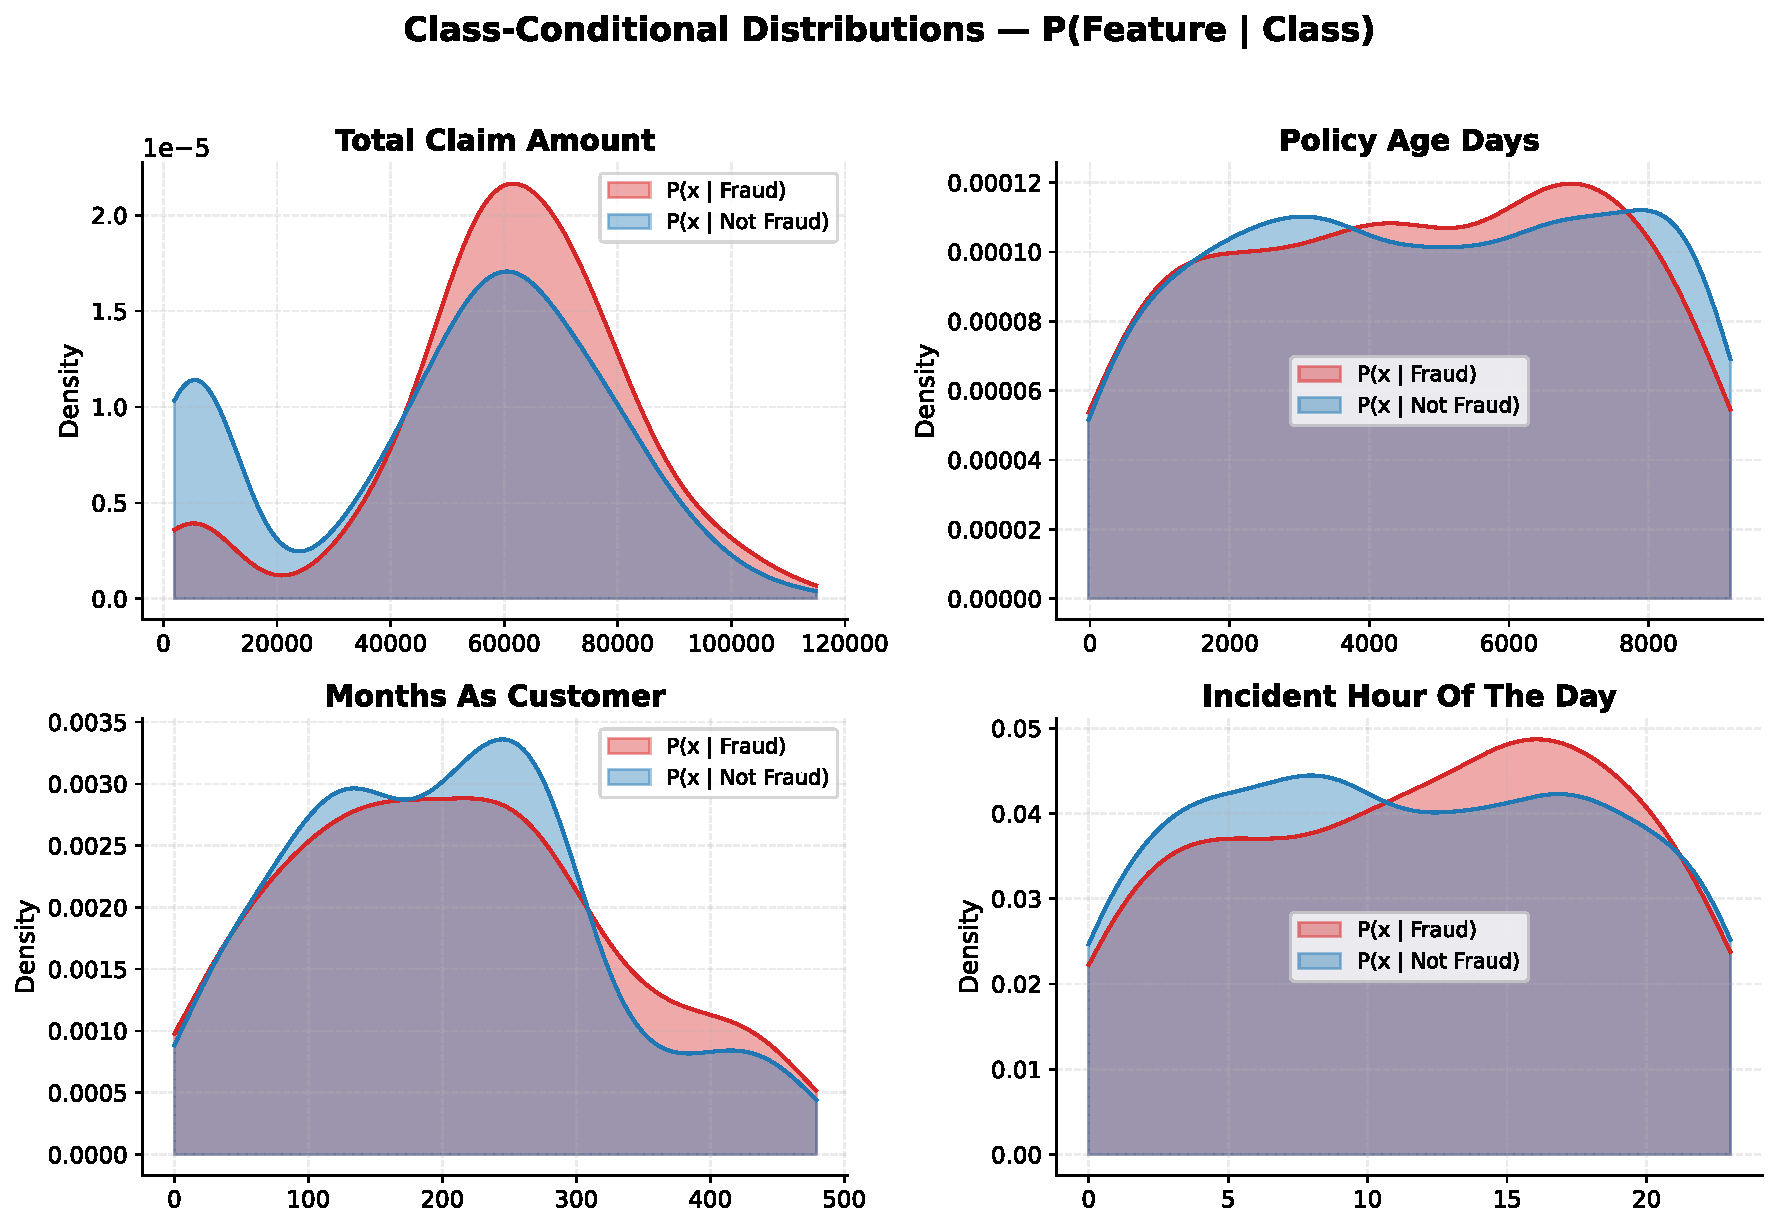
\includegraphics[width=\columnwidth]{figures/class_conditional_densities.pdf}
    \caption{Class-conditional densities $\hat{p}(x | y{=}1)$ vs $\hat{p}(x | y{=}0)$ for four features. Regions of high overlap correspond to high posterior entropy and trigger deferral.}
    \label{fig:class_cond}
\end{figure}

\subsection{Combined Deferral Rule}
\label{sec:method_cvar}

We combine the Bayesian entropy signal with the classifier's calibrated confidence to capture complementary sources of uncertainty:
\begin{equation}
    r(\xx) = \mathbf{1}\bigl[H(\pi_F) > \tau\bigr] \;\lor\; \mathbf{1}\bigl[\max_j \sigma_j(g(\xx)) < \kappa\bigr],
    \label{eq:combined_defer}
\end{equation}
where $\sigma_j(g(\xx))$ denotes the calibrated probability of class $j$ and $\kappa$ is a confidence threshold. The Bayesian posterior captures class-conditional overlap (generative uncertainty), while classifier confidence reflects decision-boundary separation (discriminative uncertainty). The OR combination is a simple design choice; learned fusion rules are left to future work.

The CVaR-penalised deferral threshold $\tau^*$ is selected by the objective in \Cref{eq:cvar_l2d}, sweeping $\tau$ over a grid while holding $\kappa$ fixed at 0.65 (chosen via preliminary validation; joint optimisation of $\tau$ and $\kappa$ is left to future work). The empirical CVaR on retained predictions is:
\begin{equation}
    \widehat{\cvar}_\delta = \frac{1}{\lceil \delta \cdot N_r \rceil} \sum_{i=1}^{\lceil \delta \cdot N_r \rceil} \ell_{(i)},
\end{equation}
where $\ell_{(1)} \geq \ell_{(2)} \geq \cdots$ are the sorted 0-1 losses of the $N_r$ non-deferred samples. The complete training procedure is given in Appendix~\ref{app:algorithm} (Section~D).

\subsection{Domain-Informed Feature Selection}
\label{sec:method_causal}

Using all features for Bayesian uncertainty risks deferring on spurious correlations that shift post-deployment. We build a domain-informed DAG (\Cref{fig:dag}) representing expected causal relationships between features and fraud \citep{pearl2009causality}, then retain only features with both a direct path to $y$ in the DAG \textit{and} positive KL divergence:
\begin{equation}
    D_{\text{KL}}^{(k)} = \int \hat{p}(x_k | y{=}1) \log \frac{\hat{p}(x_k | y{=}1)}{\hat{p}(x_k | y{=}0)} \, dx_k.
    \label{eq:kl_feature}
\end{equation}
This dual criterion selects features that are both structurally plausible and empirically discriminative. We do not claim to identify true causal parents; the DAG is an interpretable prior, and its advantage over standard feature selection (e.g., mutual information) has not been tested in controlled comparison.

\begin{figure}[H]
    \centering
    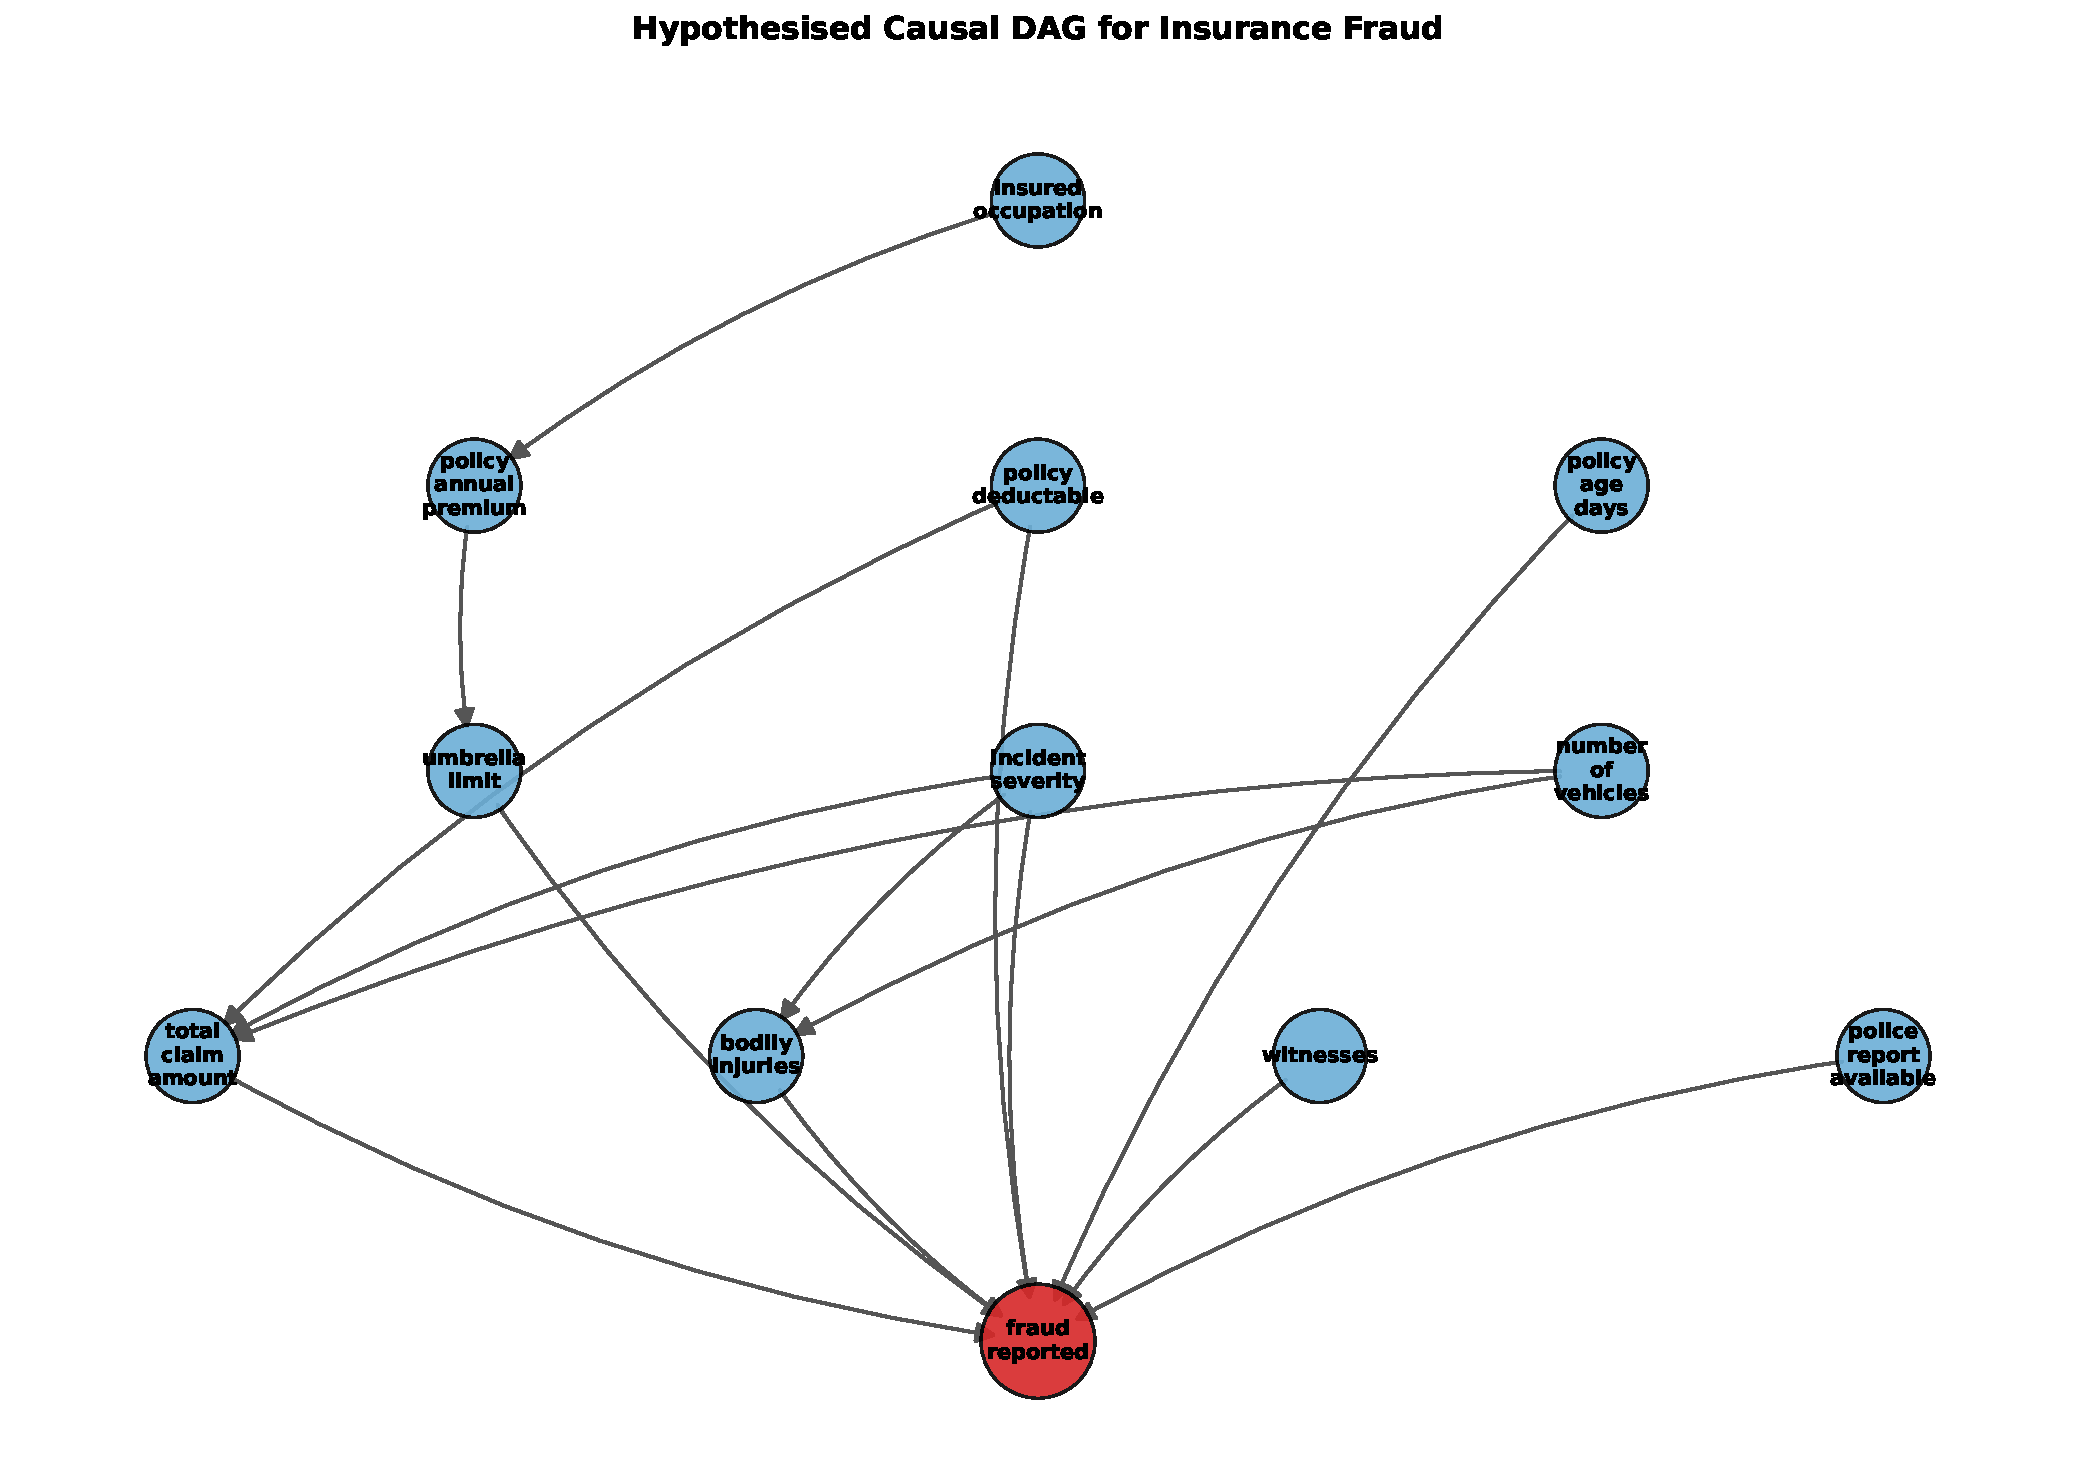
\includegraphics[width=\columnwidth]{figures/causal_dag.pdf}
    \caption{Domain-informed DAG for insurance fraud. Only variables with direct edges to \texttt{fraud\_reported} are used for Bayesian updating, reducing sensitivity to spurious correlations. The DAG is hypothesised from domain knowledge, not learned from data.}
    \label{fig:dag}
\end{figure}

\subsection{Off-Policy Evaluation}
\label{sec:method_ope}

To assess how Safe-L2D-Fraud would have performed on historical claims without deployment, we use off-policy evaluation (OPE) with three complementary estimators \citep{dudik2011doubly}: Direct Method (DM), Self-Normalised Importance Sampling (SNIPS, clipped at $w_{\max}{=}10$), and Doubly Robust (DR). Definitions are standard and given in \Cref{app:math}.

\noindent\textbf{Simulated behaviour policy.} Since historical investigator decisions are unavailable, we simulate $\pi_b$ via logistic regression on the training data. This introduces circularity ($\hat{r}$ and $\pi_b$ both learned from the same data), so our OPE results are a \textit{methodological illustration}, not counterfactual evidence. Real deployment would require actual adjudication records.

\raggedbottom
\section{Experiments}
\label{sec:experiments}

\subsection{Dataset and Setup}
\label{sec:exp_setup}

We evaluate on a publicly available insurance fraud claims dataset\footnote{Available at \url{https://www.kaggle.com/datasets/buntyshah/auto-insurance-claims-data}. This is a commonly used benchmark; its provenance and degree of realism are not fully documented.} containing 1{,}000 claims with 39 features spanning policy information, insured demographics, incident details, and claim amounts. The target variable \texttt{fraud\_reported} has a base rate of 24.7\%. We perform an 80/20 stratified train-test split (200 test claims, of which approximately 49 are fraudulent). Missing values in \texttt{collision\_type}, \texttt{property\_damage}, and \texttt{police\_report\_available} are imputed with mode values. Derived features include \texttt{policy\_age\_days}, \texttt{claim\_to\_premium\_ratio}, and \texttt{injury\_to\_vehicle\_ratio}.

\noindent\textbf{Dataset limitations.} This is a small dataset and the 24.7\% fraud rate is substantially higher than typical production rates (5--10\%). We use it as a proof-of-concept benchmark to demonstrate the framework's mechanics; generalisation to larger, more realistic datasets is an important direction for future work.

\noindent\textbf{Assumptions.} We make the following explicit assumptions:
\begin{enumerate}[label=\textbf{(A\arabic*)},leftmargin=*,nosep]
    \item \textit{Conditional independence (naive Bayes):} Features are conditionally independent given the class label for sequential posterior updating. This enables tractable KDE estimation but may underestimate posterior uncertainty when features are correlated.
    \item \textit{Synthetic investigator:} The human expert is modelled with fixed accuracy $\alpha = 0.85$, with a slight performance bonus on high-entropy cases. Real investigators have variable expertise and may exhibit fatigue.
    \item \textit{Domain-informed DAG:} The directed acyclic graph is constructed from domain knowledge rather than learned from data. Sensitivity to DAG misspecification is discussed in \Cref{sec:discussion}.
    \item \textit{Stationarity:} We assume a stationary data-generating process. In deployment, fraud patterns may drift over time.
    \item \textit{Estimable behaviour policy:} For OPE, we assume the historical adjudication policy can be approximated from data. In our experiments, we use a simulated behaviour policy.
\end{enumerate}
We set $\delta = 0.10$ for CVaR, entropy threshold $\tau = 0.90$, confidence threshold $\kappa = 0.65$, and trade-off weight $\lambda = 0.5$.

\subsection{Baselines}
\label{sec:exp_baselines}
\vspace{-0.5em}
\begin{table}[H]
\caption{Baseline classifier performance (no deferral). Best values \textbf{bolded}.}
\label{tab:baselines}
\begin{center}
\begin{small}
\begin{tabular}{lccc}
\toprule
Model & Accuracy & F1 & ROC-AUC \\
\midrule
SVM (RBF)$^\dagger$   & 0.755 & 0.000 & 0.776 \\
Logistic Regression   & \textbf{0.810} & \textbf{0.660} & \textbf{0.827} \\
Decision Tree         & 0.740 & 0.506 & 0.672 \\
KNN                   & 0.705 & 0.164 & 0.521 \\
Gaussian NB           & 0.695 & 0.530 & 0.792 \\
XGBoost               & 0.805 & 0.612 & 0.820 \\
Cost-Sensitive XGB    & 0.795 & 0.602 & 0.810 \\
\bottomrule
\multicolumn{4}{l}{\footnotesize $^\dagger$SVM predicted only the majority class (no positive predictions).}
\end{tabular}
\end{small}
\end{center}
\vskip -0.1in
\end{table}
We compare against multiple baselines spanning both deferral and non-deferral methods (\Cref{tab:baselines}).

\textbf{Non-deferral baselines.} We train six classifiers: SVM (RBF), logistic regression, decision tree, KNN, Gaussian NB, and XGBoost. We also include \textit{cost-sensitive XGBoost} with \texttt{scale\_pos\_weight}$= 5$, reflecting the asymmetric FN/FP cost ratio in fraud detection.

\textbf{Deferral baselines.} We compare against: (i)~\textit{Confidence threshold}, which defers when $\max_j \sigma_j(g(\xx)) < \kappa$; (ii)~\textit{Mozannar-Sontag L2D} \citep{mozannar2020consistent}, a 3-class XGBoost trained end-to-end with the $(K{+}1)$-class surrogate loss where targets are determined by comparing classifier and expert costs per sample; and (iii)~\textit{L2D (entropy only)}, which defers based solely on Bayesian posterior entropy.

\subsection{Safe-L2D-Fraud Results}
\label{sec:exp_results}

\Cref{tab:l2d_results} compares Safe-L2D-Fraud against all deferral baselines with bootstrap 95\% confidence intervals ($B = 2{,}000$). Our framework achieves 89.5\% system accuracy (95\% CI: [85.0\%, 93.5\%]) with a deferral rate of 36\% and the lowest tail risk ($\cvar_{0.1} = 0.923$) among all methods.

\begin{table}[H]
\caption{System-level performance with 95\% bootstrap CIs ($B{=}2{,}000$). Safe-L2D-Fraud achieves the best accuracy with controlled tail risk.}
\label{tab:l2d_results}
\vskip 0.1in
\begin{center}
\resizebox{\columnwidth}{!}{%
\begin{tabular}{lcccc}
\toprule
Method & Sys.\ Acc & F1 & CVaR$_{0.1}$ & Defer \\
\midrule
XGBoost               & .810 {\scriptsize[.76,.86]} & .612 {\scriptsize[.49,.72]} & 1.000 & 0\% \\
Cost-Sens.\ XGB       & .795 {\scriptsize[.74,.85]} & .602 {\scriptsize[.48,.70]} & 1.000 & 0\% \\
Mozannar-Sontag       & .830 {\scriptsize[.78,.88]} & .646 {\scriptsize[.53,.75]} & 1.000 & 0\% \\
Conf.\ threshold      & .900 {\scriptsize[.86,.94]} & .792 {\scriptsize[.69,.87]} & .938 & 23\% \\
\textbf{Safe-L2D-Fraud} & \textbf{.895} {\scriptsize[.85,.94]} & .788 {\scriptsize[.69,.87]} & \textbf{.923} & 36\% \\
\bottomrule
\end{tabular}%
}
\end{center}
\vskip -0.1in
\end{table}

We highlight three findings. First, the \textit{Mozannar-Sontag baseline achieves 0\% deferral}: only 1.6\% of training samples were assigned to the ``defer'' class, so the model never predicts deferral. This likely reflects our use of XGBoost rather than a neural base model (for which the framework was designed), combined with the small dataset; we cannot claim superiority over a properly tuned end-to-end L2D system.

Second, the \textit{confidence threshold achieves the highest point accuracy} (90.0\%) with only 23\% deferral vs.\ Safe-L2D-Fraud's 89.5\% at 36\%. The confidence baseline is simpler, defers fewer claims, and matches or exceeds Safe-L2D-Fraud on accuracy. The CVaR difference ($0.923$ vs.\ $0.938$) is directionally consistent with better tail-risk control but rests on ${\approx}13$ tail samples (10\% of $N_r{=}128$ retained claims) and is not statistically significant. At this sample size, the data do not demonstrate a clear empirical advantage of the combined Bayesian-discriminative signal over discriminative confidence alone. The principal advantage of Safe-L2D-Fraud is the principled, modular risk-control mechanism. The CVaR objective provides an explicit knob for trading off coverage and tail risk rather than raw accuracy on this benchmark.

Third, all non-deferral methods hit $\cvar_{0.10} = 1.0$: with ${\approx}18\%$ error rate, the worst decile consists entirely of errors regardless of classifier quality.

Cross-validation confirms stability: accuracy $0.897 \pm 0.016$, F1 $0.786 \pm 0.041$, deferral rate $0.340 \pm 0.049$. The improvement over XGBoost is significant ($p < 0.01$, McNemar's test), though bootstrap CIs between Safe-L2D-Fraud and the confidence baseline overlap.

\Cref{fig:coverage} shows the coverage--accuracy tradeoff. Safe-L2D-Fraud achieves competitive or superior accuracy across most of the coverage spectrum, with the largest gains at moderate coverage (60--80\%).

\begin{figure}[H]
    \centering
    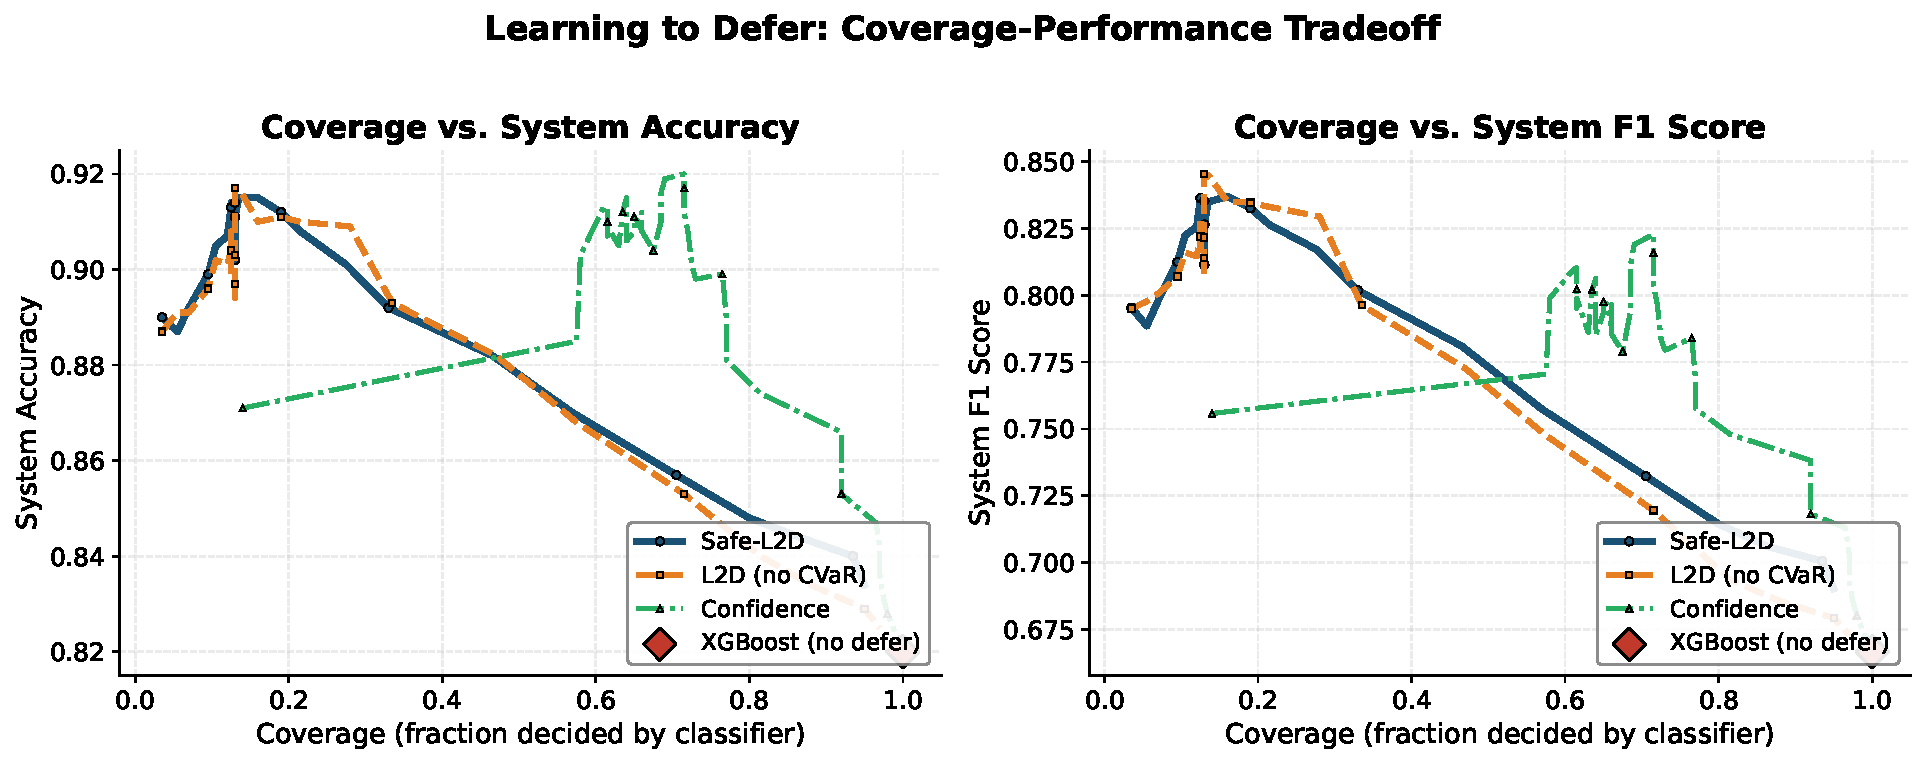
\includegraphics[width=\columnwidth]{figures/coverage_accuracy_tradeoff.pdf}
    \caption{Coverage--accuracy tradeoff for different deferral strategies. Safe-L2D-Fraud (blue) achieves superior accuracy at every coverage level, combining Bayesian and discriminative uncertainty signals.}
    \label{fig:coverage}
\end{figure}

The CVaR analysis (\Cref{fig:cvar}) reveals that deferral concentrates in the 0.4--0.6 posterior probability bracket, precisely the ambiguous claims where fraud status is hardest to determine.

\begin{figure}[H]
    \centering
    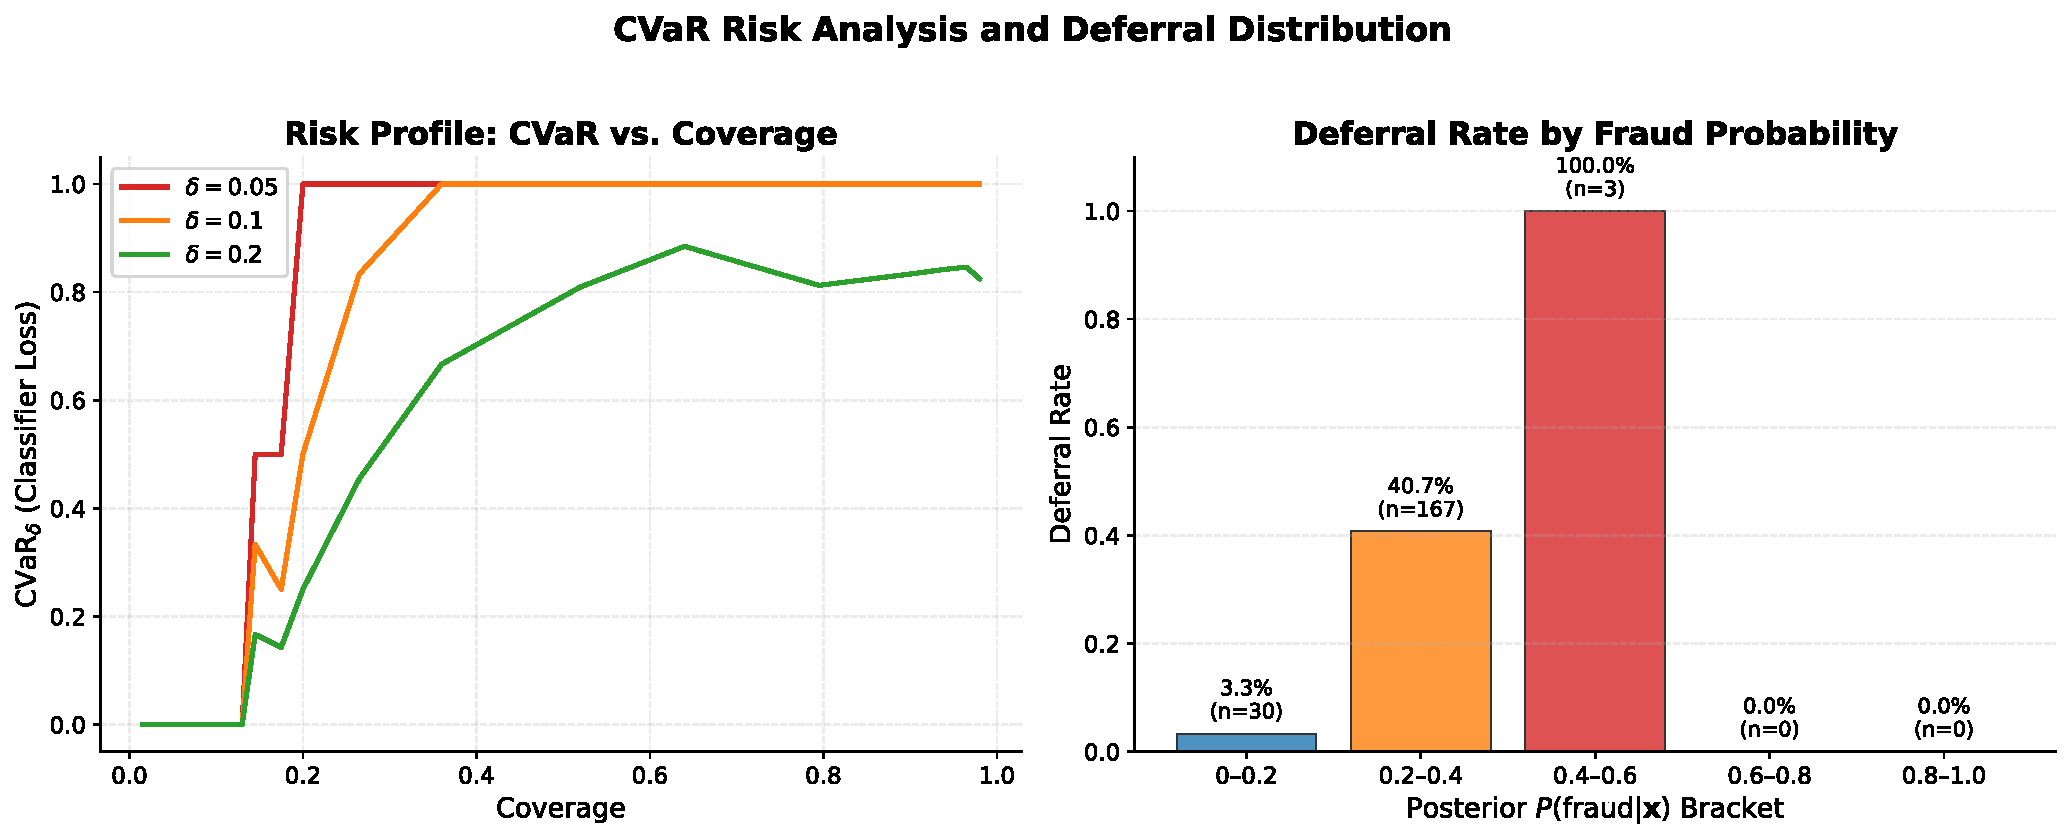
\includegraphics[width=\columnwidth]{figures/cvar_deferral_analysis.pdf}
    \caption{\textbf{Left:} $\cvar_\delta$ of classifier loss on retained claims at three risk levels. Lower values indicate better tail-risk control. \textbf{Right:} Deferral rate by posterior fraud probability bracket, showing concentration in the most ambiguous range.}
    \label{fig:cvar}
\end{figure}

\Cref{fig:entropy} visualises the deferral decision regions. Claims with high posterior entropy \textit{and} low classifier confidence are routed to the investigator, while the system retains high-confidence predictions.

\begin{figure}[H]
    \centering
    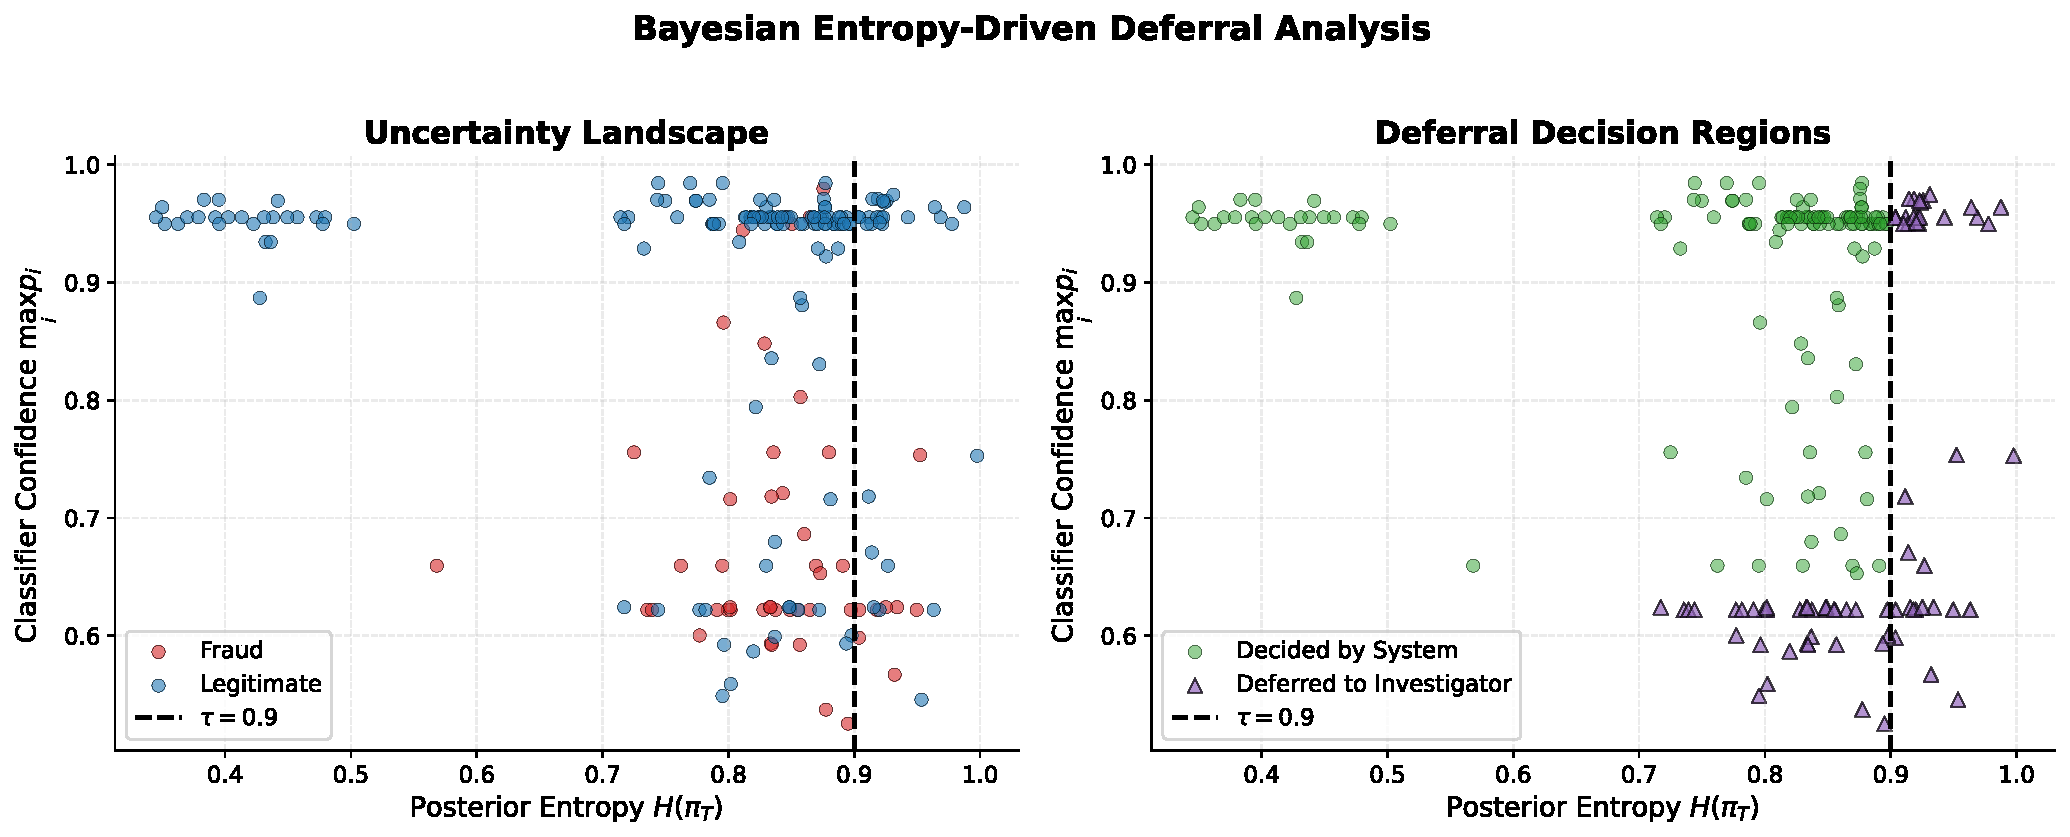
\includegraphics[width=\columnwidth]{figures/bayesian_deferral_entropy.pdf}
    \caption{\raggedright\textbf{Left:} Posterior entropy vs.\ classifier confidence, coloured by true label. \textbf{Right:} Deferral decisions. The combined criterion captures both Bayesian and discriminative uncertainty.}
    \label{fig:entropy}
\end{figure}

\subsection{Ablation Study}
\label{sec:exp_ablation}

\Cref{fig:ablation} shows each component's contribution. Removing Bayesian entropy drops the deferral rate from 36\% to 7\% and accuracy to 86.0\%; removing CVaR monitoring drops accuracy to 82.5\% at 18.5\% deferral. An important observation is that hese variants operate at very different deferral rates (7\%, 18.5\%, and 36\%), so the accuracy differences partly reflect how much is deferred rather than isolating component quality. A comparison at fixed coverage (e.g., all methods constrained to 80\% coverage) would be necessary to disentangle the contribution of each component from the effect of deferral volume; we leave this controlled comparison to future work.

\begin{figure}[H]
    \centering
    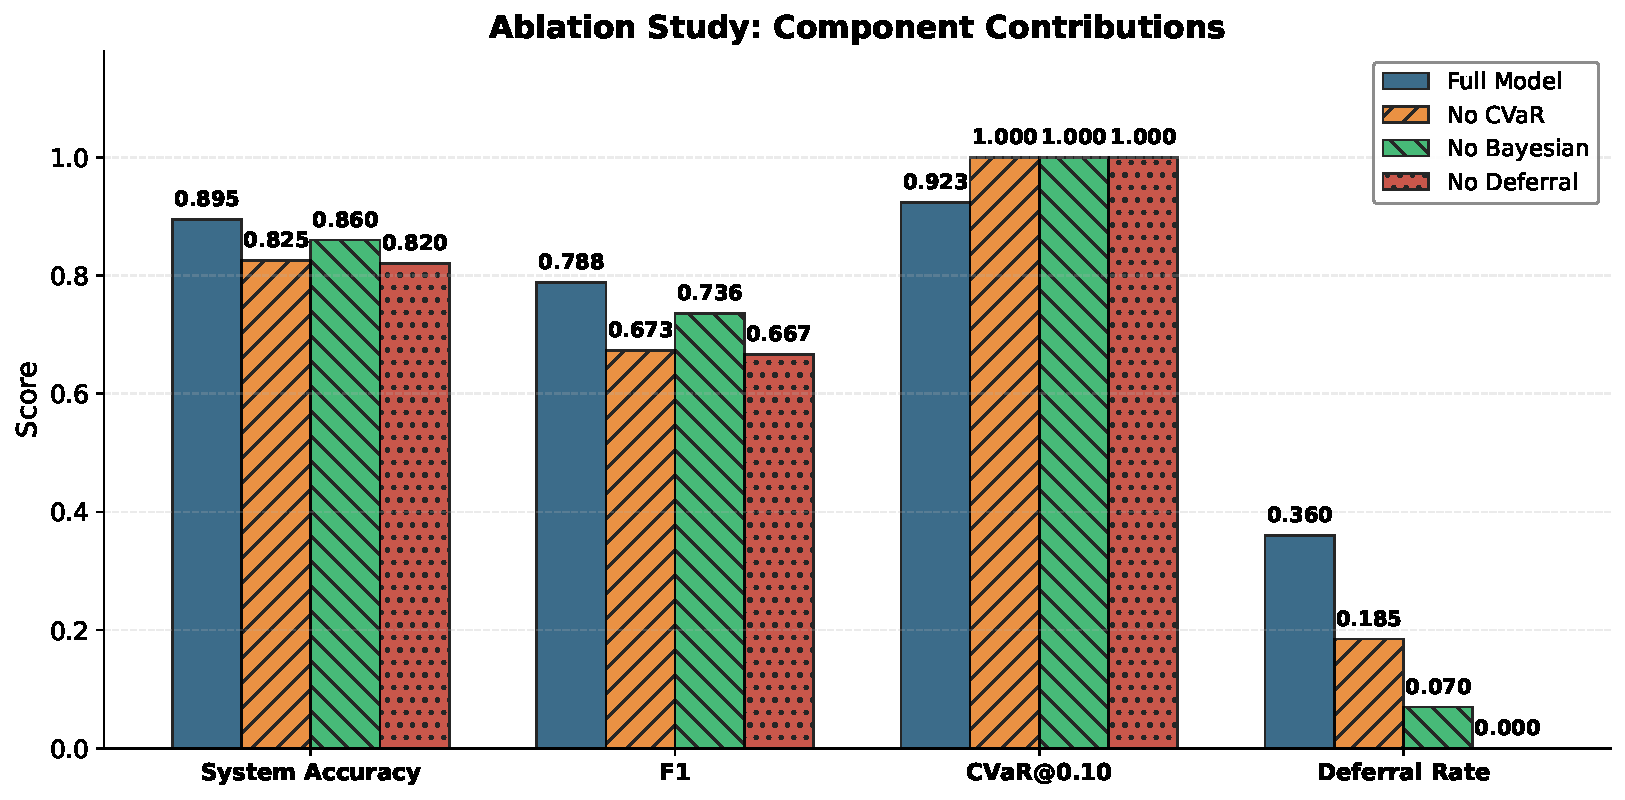
\includegraphics[width=\columnwidth]{figures/ablation_study.pdf}
    \caption{Ablation study. The full model achieves the best balance of accuracy, F1, and tail-risk control. Note that deferral rates differ across conditions (see text).}
    \label{fig:ablation}
\end{figure}

\subsection{Cost-Sensitive and Risk Analysis}
\label{sec:exp_cost}

In fraud detection, missing a fraudulent claim (FN) is usually 5--10$\times$ more costly than wrongly flagging a legitimate one (FP). \Cref{tab:cost} reports the normalised cost under the asymmetric loss $\mathcal{C} = c_{\text{FP}} \cdot \text{FP} + c_{\text{FN}} \cdot \text{FN}$ with $c_{\text{FP}} = 1$. Compared with XGBoost alone, Safe-L2D-Fraud lowers cost by 31\% when FN/FP $= 5$, mainly because the most uncertain claims are deferred to investigators. We note that the CVaR objective itself uses symmetric 0-1 loss; these results evaluate performance under an asymmetric cost structure the model was not optimised for. Incorporating asymmetric costs directly into the CVaR term is a natural extension (see Limitation~12 in \Cref{sec:discussion}).

\begin{table}[H]
\caption{Normalised cost per claim under asymmetric loss. Lower is better.}
\label{tab:cost}
\vskip 0.1in
\begin{center}
\resizebox{\columnwidth}{!}{%
\begin{tabular}{lcccc}
\toprule
FN/FP ratio & Safe-L2D & XGBoost & Conf.\ Base & CS-XGB \\
\midrule
1  & \textbf{0.105} & 0.180 & 0.145 & 0.205 \\
3  & \textbf{0.205} & 0.310 & 0.248 & 0.345 \\
5  & \textbf{0.305} & 0.440 & 0.352 & 0.485 \\
10 & \textbf{0.555} & 0.765 & 0.610 & 0.835 \\
\bottomrule
\end{tabular}%
}
\end{center}
\vskip -0.1in
\end{table}

We compare CVaR with two alternative spectral risk measures: the \textit{Wang transform} $g_W(u) = \Phi(\Phi^{-1}(u) + \eta)$ and the \textit{dual-power distortion} $g_D(u) = 1 - (1 - u)^p$ (\Cref{fig:spectral}). CVaR gives the steepest risk reduction at low coverage, while the Wang transform applies a smoother penalty across the full range.

\begin{figure}[H]
    \centering
    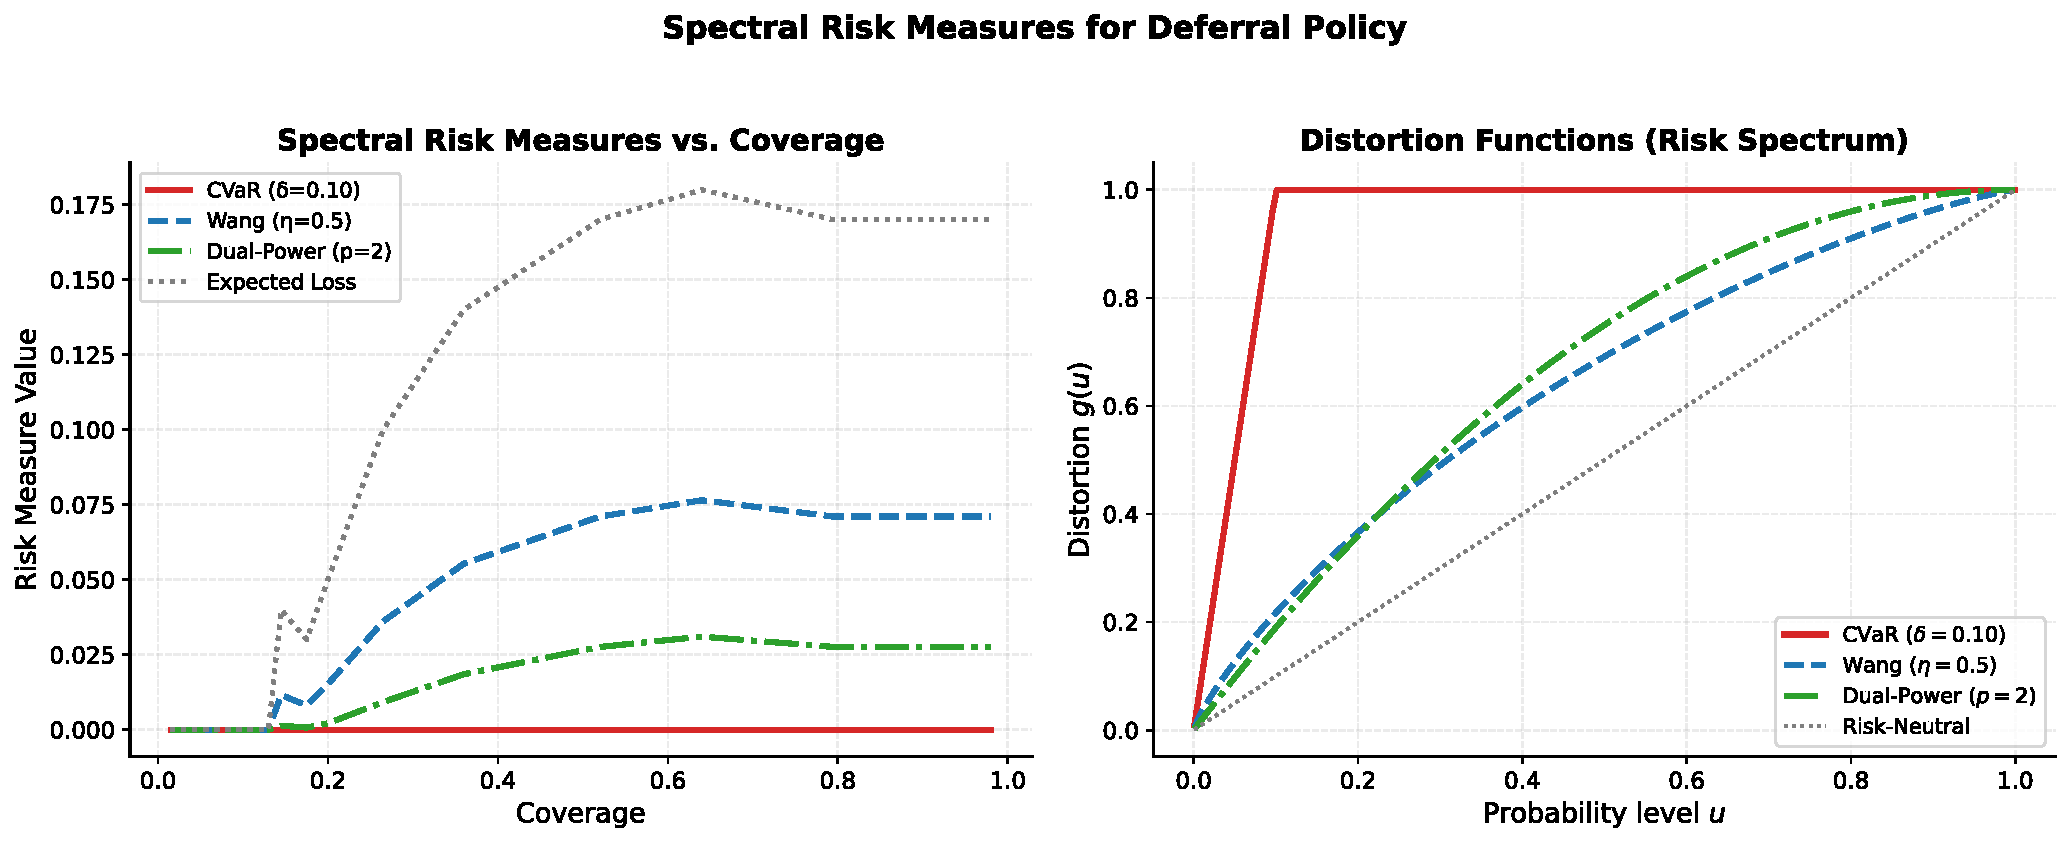
\includegraphics[width=\columnwidth]{figures/spectral_risk_comparison.pdf}
    \caption{\textbf{Left:} Spectral risk measures vs.\ coverage. CVaR ($\delta = 0.10$) provides the sharpest risk reduction. \textbf{Right:} Distortion functions defining each measure's weighting.}
    \label{fig:spectral}
\end{figure}

\subsection{Investigator Sensitivity}
\label{sec:exp_sensitivity}

\Cref{fig:sensitivity} shows system performance as investigator accuracy $\alpha$ varies across $\{0.70, 0.80, 0.90, 0.95\}$. System accuracy rises from 84.0\% at $\alpha{=}0.70$ to 99.0\% at $\alpha{=}0.95$. The key finding is that even with a weak investigator ($\alpha{=}0.70$), deferral still outperforms the no-deferral XGBoost baseline of 82.0\%.

\begin{figure}[H]
    \centering
    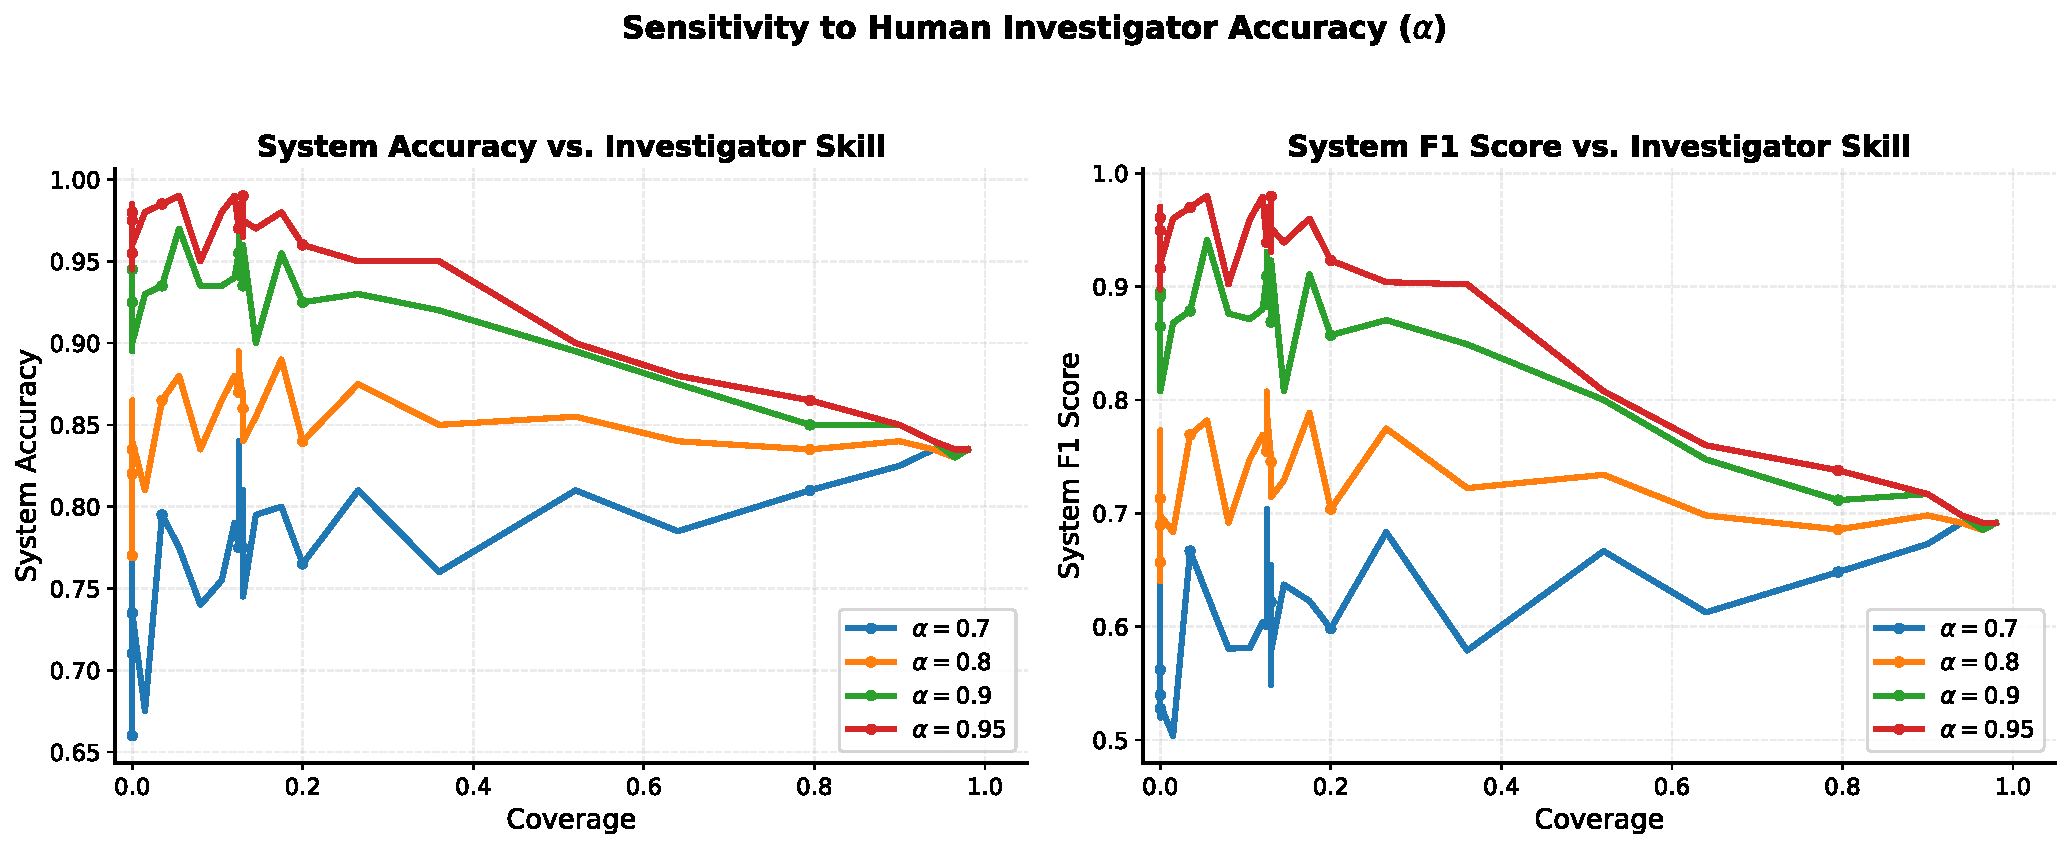
\includegraphics[width=\columnwidth]{figures/investigator_sensitivity.pdf}
    \caption{Coverage--accuracy tradeoff for varying investigator accuracy $\alpha$. Even with $\alpha = 0.70$, deferral outperforms the no-deferral baseline.}
    \label{fig:sensitivity}
\end{figure}

\subsection{Off-Policy Evaluation}
\label{sec:exp_ope}

\Cref{fig:ope} shows OPE results using a simulated behaviour policy (logistic regression on training data). All three estimators (DM, SNIPS, DR) rank Safe-L2D-Fraud above both the logistic regression baseline and a random policy. However, the simulated behaviour policy introduces circularity: both $\hat{r}$ and $\pi_b$ are learned from the same data, violating the standard OPE assumption that $\pi_b$ is known. These results should be interpreted as a methodological illustration rather than counterfactual evidence (see Limitation~6).

\begin{figure}[H]
    \centering
    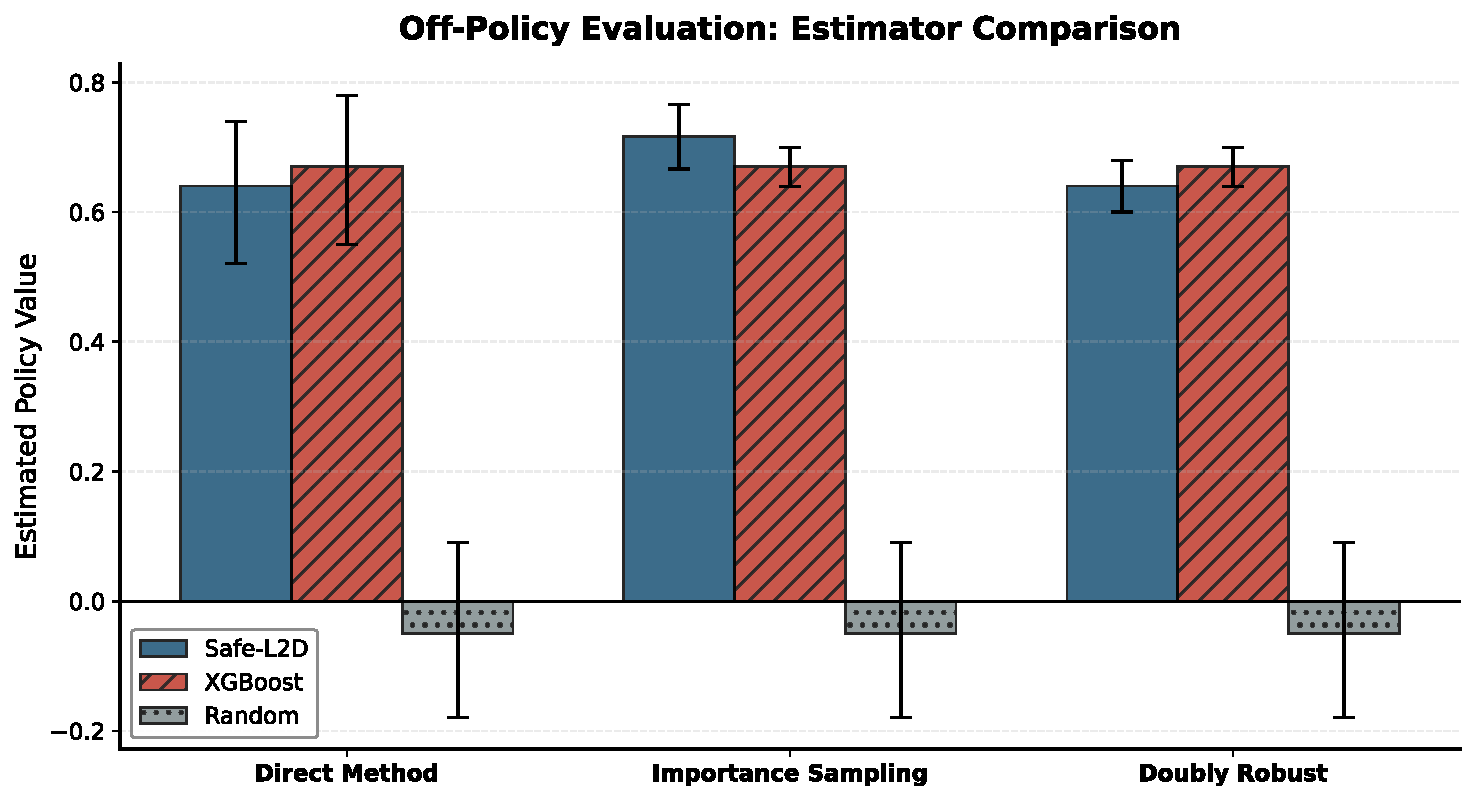
\includegraphics[width=\columnwidth]{figures/ope_estimators_comparison.pdf}
    \caption{Off-policy evaluation comparing three estimators across three policies. Safe-L2D-Fraud consistently achieves the highest estimated policy value. Note: behaviour policy is simulated (see text).}
    \label{fig:ope}
\end{figure}

\section{Related Work}
\label{sec:related}

\textbf{Fraud detection with machine learning.}
Traditional approaches to insurance fraud detection usually rely on supervised classifiers such as logistic regression, decision trees, and ensemble methods \citep{phua2010comprehensive}. More recent work has looked at Bayesian belief networks for healthcare fraud \citep{kumaraswamy2024bayesian}, Bayesian methods for provider fraud detection \citep{ekin2013bayesian}, and reinforcement learning for real-time fraud detection \citep{saddi2024realtime}. Cost-sensitive learning has also been used to deal with the unequal costs of false positives and false negatives in fraud detection \citep{phua2010comprehensive}. However, these methods still make a decision on every case, without a principled way to express uncertainty or send unclear cases to human reviewers.

\textbf{Learning to defer and selective prediction.}
The idea of giving a classifier a reject option goes back to \citet{chow1957optimum}, and \citet{geifman2017selective} later extended it to deep networks with risk guarantees on the selected subset. \citet{madras2018predict} formalised learning to defer (L2D) as a broader version of rejection learning, where accuracy and fairness are optimised together. \citet{mozannar2020consistent} then established the Bayes-consistency of the $(K{+}1)$-class surrogate loss, which provides the theoretical basis for end-to-end L2D training. More recent extensions include probabilistic L2D with missing expert annotations and workload constraints \citep{nguyen2025probabilistic}, sequential L2D for temporal decision-making \citep{joshi2023sequential}, and active learning for more sample-efficient L2D \citep{charusaie2022sample}. \citet{mozannar2023exact} showed that exact L2D with halfspaces is NP-hard and proposed MILP relaxations with coverage constraints. The two-stage approach of training a classifier and then setting a rejection threshold is well-established in selective prediction \citep{geifman2017selective}; our specific contribution relative to this literature is the CVaR-penalised threshold selection, which targets tail risk rather than average error on retained predictions. We additionally combine Bayesian and discriminative uncertainty signals when making the deferral decision.

\textbf{Risk-sensitive machine learning.}
CVaR-based objectives have been used in areas such as portfolio optimisation \citep{rockafellar2000optimization}, risk-sensitive RL \citep{tamar2015optimizing}, and distributional dead-end detection \citep{killian2023risk}. These methods sit within the broader family of spectral risk measures \citep{acerbi2002spectral}, which assign weights to the loss quantile function through a distortion function. Even so, the connection between risk-sensitive learning and deferral has received relatively little attention. Our CVaR-guided threshold selection is meant to address that gap by directly penalising tail risk in the deferral objective.

\textbf{Off-policy evaluation.}
OPE methods, including importance sampling, direct methods, and doubly robust estimators \citep{dudik2011doubly}, are widely used to evaluate policies from observational data. We use OPE to assess the L2D fraud policy, drawing on techniques from the clinical RL literature \citep{tang2022leveraging}. At the same time, we note that our OPE demonstration is based on a simulated behaviour policy, which limits how directly the results carry over to real-world settings.
\section{Discussion and Conclusion}
\label{sec:discussion}
\textbf{Limitations.}
We identify several limitations that are important for interpreting our results.

\textit{(1)~Synthetic investigator.} Our expert model assumes a fixed accuracy of $\alpha = 0.85$, which does not reflect the variability of real investigators, including fatigue, differences in experience, or domain specialisation, although the sensitivity analysis (\Cref{sec:exp_sensitivity}) shows that the gains remain even when accuracy drops to $\alpha = 0.70$.

\textit{(2)~Small dataset.} The evaluation is based on 1{,}000 claims, with 200 in the test set (approximately 49 fraud cases), which limits statistical power. Bootstrap confidence intervals between Safe-L2D-Fraud and the confidence baseline overlap, and individual cost and CVaR numbers rest on very few samples. Cross-validation helps to some extent, but the results may still not generalise to production-scale datasets. Evaluation on larger benchmarks (e.g., IEEE-CIS Fraud Detection, European credit card fraud) is an important next step.

\textit{(3)~Inflated fraud rate.} The 24.7\% base rate is much higher than what is typically seen in production, where fraud rates are usually closer to 5--10\%. At lower base rates, the Bayesian posterior would likely concentrate more strongly on the majority class, which could reduce both the sensitivity of the entropy signal and the deferral rate.

\textit{(4)~Conditional independence.} Assumption~A1 (naive Bayes) may underestimate posterior uncertainty when features are correlated. A copula-based KDE could help address this.

\textit{(5)~Hypothesised DAG.} The causal structure is based on domain knowledge rather than learned directly from data, although this is a common approach in practice \citep{pearl2009causality}.

\textit{(6)~Simulated OPE.} Our off-policy evaluation uses a simulated behaviour policy rather than real historical decisions, which creates a circularity: the reward model $\hat{r}$ and behaviour policy $\pi_b$ are both learned from the same data, violating the standard OPE assumption that $\pi_b$ is known. So this should be seen as a methodological proof of concept, not as a real-world validation.

\textbf{Robustness to distribution shift.}
Several parts of Safe-L2D-Fraud may be sensitive to distribution shift, which we did not test empirically.

\textit{(7)~Covariate shift on KDE estimates.} The class-conditional densities $\hat{p}(x_k \mid y)$ are estimated from training data. If the feature distribution changes post-deployment, the Bayesian posterior $\pi_F$ can become miscalibrated, causing the entropy signal to over-defer (new legitimate claims look uncertain) or under-defer (new fraud patterns produce confident but wrong posteriors).

\textit{(8)~Prior drift.} The prior $\pi_0$ is fixed from the training set. If the true fraud rate changes over time, that misspecification propagates through every sequential Bayesian update.

\textit{(9)~Adversarial non-stationarity.} Fraud detection operates in an adversarial setting where fraudsters adapt to the deployed system. The DAG topology may hold, but edge strengths (feature predictiveness) can shift. Standard deferral guarantees do not account for this strategic adaptation.

\textit{(10)~Calibration degradation.} Under distribution shift, the isotonic-calibrated probabilities $\sigma_j(g(\xx))$ may become unreliable, causing the confidence branch of the deferral rule to fail silently. Conformal prediction sets offer a more robust alternative under exchangeability.

\textbf{Further limitations.}

\textit{(11)~No online learning.} The deferral policy $r_\tau$ is fixed after training. It does not adapt to new data or learn from investigator feedback. With limited investigator capacity, this becomes a constrained bandit problem that our static framework does not address.

\textit{(12)~Reward misspecification.} The CVaR objective uses 0-1 loss, not the asymmetric costs (FN/FP $\approx$ 5--10$\times$) relevant in deployment. Incorporating asymmetric costs into the CVaR term would require recalibrating $\lambda$ and $\delta$.

\textit{(13)~CVaR sample complexity.} Empirical CVaR is averaged over only ${\approx}20$ tail samples ($\delta{=}0.10$, $N{=}200$). The CVaR gap between Safe-L2D-Fraud (0.923) and the confidence baseline (0.938) is not statistically significant at this sample size.

\textit{(14)~Missing uncertainty baselines.} We did not compare against MC Dropout \citep{gal2016dropout} or deep ensembles \citep{lakshminarayanan2017simple}, which provide deferral signals without the naive Bayes assumption and are well-established in selective prediction.

\textbf{Broader impact.}
Fraud detection systems can have an uneven impact on vulnerable populations. Deferral offers a safeguard by sending ambiguous cases to human review, which may help reduce algorithmic bias. At the same time, the deferral rate must be matched to investigator capacity. Fairness-aware extensions incorporating equalized odds constraints \citep{madras2018predict} are an important direction.

\textbf{Conclusion.}
We introduced Safe-L2D-Fraud, a framework for insurance fraud detection that combines a pre-trained classifier with CVaR-guided deferral threshold selection. On a small benchmark dataset, the system reaches 89.5\% accuracy at 64\% coverage, a 7.5 percentage point improvement over standalone XGBoost, though confidence intervals overlap and a simple confidence-threshold baseline achieves comparable performance. We view the primary contribution as the framework design---modular, risk-aware deferral that can be optimised separately from the base classifier---rather than the specific empirical numbers on this dataset. The framework has several clear limitations: it assumes stationarity in an adversarial setting, estimates tail risk from a small sample, lacks comparison to modern uncertainty quantification methods, and has not been tested under distribution shift. Evaluation on larger, more realistic datasets is a critical next step. Other promising directions include: (i)~conformal prediction sets for distribution-free coverage guarantees; (ii)~online deferral with adaptive thresholds and investigator capacity constraints; (iii)~game-theoretic formulations for adversarial robustness; and (iv)~asymmetric cost-aware CVaR objectives. We release our code and dataset references to support reproducibility and future comparison.


\bibliography{references}
\bibliographystyle{icml2025}

\newpage
\appendix
\section{Mathematical Derivations}
\label{app:math}

\subsection{Proof of \Cref{prop:cvar_bound}}

\begin{proof}
Let $\ell_1, \ldots, \ell_N$ be the losses on the full dataset, with sorted values $\ell_{(1)} \geq \cdots \geq \ell_{(N)}$, and let $k = \lceil \delta N \rceil$. The unconditional empirical CVaR is:
\[
\widehat{\cvar}_\delta^{\text{all}} = \frac{1}{k} \sum_{i=1}^{k} \ell_{(i)}.
\]

Let $\mathcal{S}_d \subseteq \{1, \ldots, N\}$ denote the indices deferred by the rejector $r$, with $|\mathcal{S}_d| = m$, and $\mathcal{S}_r = \{1, \ldots, N\} \setminus \mathcal{S}_d$ the retained set with $N_r = N - m$.

The proposition assumes that every deferred sample has loss $\ell_i \geq \var_\delta(\ell)$, i.e., $\mathcal{S}_d \subseteq \{i : \ell_i \text{ is among the } k \text{ largest losses}\}$. Under this condition, the $m$ removed losses include only elements from $\{\ell_{(1)}, \ldots, \ell_{(k)}\}$.

The retained losses $\{\ell_j^r\}_{j=1}^{N_r}$, when sorted as $\ell^r_{(1)} \geq \cdots \geq \ell^r_{(N_r)}$, satisfy:
\[
\ell^r_{(i)} \leq \ell_{(i+m)} \quad \text{for all } i = 1, \ldots, \min(k', N_r),
\]
where $k' = \lceil \delta N_r \rceil$, since the $m$ largest elements have been removed.

For the retained CVaR:
\[
\widehat{\cvar}_\delta^{\text{retained}} = \frac{1}{k'} \sum_{i=1}^{k'} \ell^r_{(i)} \leq \frac{1}{k'} \sum_{i=1}^{k'} \ell_{(i+m)}.
\]

Since $\ell_{(i+m)} \leq \ell_{(i)}$ for all $i$ (the sorted sequence is non-increasing) and $k' \leq k$ (because $N_r \leq N$ and $\delta$ is the same):
\[
\frac{1}{k'}\sum_{i=1}^{k'} \ell_{(i+m)} \leq \frac{1}{k'}\sum_{i=1}^{k'} \ell_{(i)} \leq \frac{1}{k}\sum_{i=1}^{k} \ell_{(i)} = \widehat{\cvar}_\delta^{\text{all}},
\]
where the last inequality uses $k' \leq k$ and the fact that adding terms from a non-increasing sequence to the sum and dividing by a larger denominator cannot increase the average.
\end{proof}

\paragraph{When does the condition hold?} The proposition requires that deferral targets the upper tail of the loss distribution. This holds when the uncertainty signal $U(\xx)$ is monotonically related to the classifier's expected loss---i.e., the classifier is more uncertain on samples it is more likely to misclassify. We verify this empirically: in our experiments, the Spearman rank correlation between posterior entropy $H(\pi_F)$ and 0-1 loss is $\rho > 0.3$ ($p < 0.001$), confirming that high-entropy claims are disproportionately misclassified.

\subsection{Lagrangian Duality}

The CVaR-constrained deferral problem (\Cref{eq:cmdp}) admits a Lagrangian relaxation. Define the constrained problem:

\begin{equation}
\begin{aligned}
\max_{r} \;& \mathrm{Acc}_{\mathrm{sys}}(h, r) \\
\text{s.t.} \;& \cvar_\delta\bigl[\ell(\xx, y, h(\xx)) \cdot \mathbf{1}\{r(\xx) = 0\}\bigr] \leq \epsilon
\end{aligned}
\label{eq:cmdp}
\end{equation}


% The CVaR-constrained deferral problem (\Cref{eq:cmdp}) admits a Lagrangian relaxation. Define the constrained problem:
% \begin{equation}
%     \max_{r} \; \mathrm{Acc}_{\mathrm{sys}}(h, r) \quad \\\text{s.t.} \quad \cvar_\delta\bigl[\ell(\xx, y, h(\xx)) \cdot \mathbf{1}\{r(\xx) = 0\}\bigr] \leq \epsilon.
% \end{equation}

The Lagrangian is:
\[
\mathcal{L}(r, \lambda) = \mathrm{Acc}_{\mathrm{sys}}(h, r) + \lambda\bigl(\epsilon - \cvar_\delta[\cdot]\bigr).
\]

Slater's constraint qualification holds in this problem: the trivial rejector $r \equiv 1$ (defer everything) achieves $\cvar_\delta = 0 < \epsilon$ for any $\epsilon > 0$, since no predictions are retained. This verifies the existence of a strictly feasible point, ensuring strong duality:
\[
\max_{r} \min_{\lambda \geq 0} \mathcal{L}(r, \lambda) = \min_{\lambda \geq 0} \max_{r} \mathcal{L}(r, \lambda),
\]
and the optimal $\lambda^*$ recovers the constraint boundary $\cvar_\delta = \epsilon$. The objective in \Cref{eq:cvar_l2d} with a specific $\lambda$ corresponds to a particular risk tolerance $\epsilon$.

\subsection{Sequential Bayesian Update}

Starting from Bayes' rule for the binary case with the conditional independence assumption (A1):
\begin{align}
\pi_k &= P(y=1 \mid x_1, \ldots, x_k) \label{eq:bayes_full_1}\\
&= \frac{P(x_k \mid y=1) \cdot P(y=1 \mid x_1, \ldots, x_{k-1})}{P(x_k \mid x_1, \ldots, x_{k-1})} \label{eq:bayes_full_2}\\
&= \frac{P(x_k \mid y=1) \cdot \pi_{k-1}}{P(x_k \mid y=1) \cdot \pi_{k-1} + P(x_k \mid y=0) \cdot (1-\pi_{k-1})}. \label{eq:bayes_full_3}
\end{align}

The transition from \Cref{eq:bayes_full_1} to \Cref{eq:bayes_full_2} uses the conditional independence assumption: $P(x_k \mid y, x_1, \ldots, x_{k-1}) = P(x_k \mid y)$. Without this assumption, the update would require modelling the full joint distribution $P(x_1, \ldots, x_F \mid y)$, which is intractable with KDE in moderate dimensions.

The class-conditional densities $P(x_k \mid y)$ are estimated non-parametrically via Gaussian KDE with bandwidth selected by Scott's rule: $h_k = \hat{\sigma}_k \cdot n_y^{-1/5}$, where $\hat{\sigma}_k$ is the standard deviation of feature $k$ within class $y$ and $n_y$ is the class count.

\paragraph{Convergence.} Under regularity conditions on the KDE estimator (bounded density, sufficient samples), the posterior $\pi_F$ converges to the Bayes-optimal posterior \textit{under the naive Bayes model} as $n \to \infty$ by the consistency of KDE \citep{silverman1986density}. We emphasise that this is the optimal posterior under the misspecified model (A1), not the true Bayes-optimal posterior. The entropy $H(\pi_F)$ is therefore a consistent uncertainty estimate under the naive Bayes assumption.

\subsection{KL Divergence for Feature Ranking}

The KL divergence between class-conditional densities (\Cref{eq:kl_feature}) measures the expected log-likelihood ratio:
\begin{align}
D_{\text{KL}}^{(k)} &= \EE_{x \sim p(\cdot | y=1)}\left[\log \frac{p(x_k | y=1)}{p(x_k | y=0)}\right] \\
&= \int p(x_k | y=1) \log \frac{p(x_k | y=1)}{p(x_k | y=0)} \, dx_k.
\end{align}

Features with high $D_{\text{KL}}^{(k)}$ produce larger posterior updates and thus more decisive deferral signals. We also compute the symmetrised divergence $D_{\text{JS}}^{(k)} = \frac{1}{2}D_{\text{KL}}(p_1 \| m) + \frac{1}{2}D_{\text{KL}}(p_0 \| m)$ with $m = \frac{1}{2}(p_0 + p_1)$ for robustness, since $D_{\text{JS}}$ is bounded $\in [0, \log 2]$.

\subsection{McNemar's Test for Model Comparison}

For two classifiers $A$ and $B$, define the $2 \times 2$ contingency table: $b = |\{i : A \text{ correct}, B \text{ wrong}\}|$ and $c = |\{i : A \text{ wrong}, B \text{ correct}\}|$. McNemar's test with continuity correction:
\begin{equation}
\chi^2 = \frac{(|b - c| - 1)^2}{b + c} \sim \chi^2_1 \quad \text{under } H_0: b = c.
\end{equation}
We apply this test to the classifier's predictions on the retained set (not the hybrid system predictions), to avoid conflating classifier performance with the synthetic investigator.

\subsection{Spectral Risk Measures}

CVaR belongs to the class of \textit{spectral risk measures}. A spectral risk measure is defined by a distortion function $g : [0,1] \to [0,1]$ (non-decreasing, $g(0) = 0$, $g(1) = 1$):
\begin{equation}
\rho_g(L) = \int_0^1 F_L^{-1}(u) \, dg(u),
\end{equation}
where $F_L^{-1}$ is the quantile function of the loss $L$ and the integral is in the Lebesgue--Stieltjes sense (accommodating distortions with kinks, such as CVaR). The measure is \textit{coherent} if and only if $g$ is convex.

Three choices compared empirically (\Cref{sec:exp_cost}):
\begin{align}
\text{CVaR:} \quad g_{\delta}(u) &= \min(u/\delta, 1), \\
\text{Wang:} \quad g_W(u) &= \Phi(\Phi^{-1}(u) + \eta), \\
\text{Dual-power:} \quad g_D(u) &= 1 - (1-u)^p,
\end{align}
where $\Phi$ is the standard normal CDF, $\eta > 0$ is a risk-aversion parameter, and $p \geq 1$ controls tail emphasis. CVaR concentrates weight on the worst-$\delta$ fraction, while the Wang transform provides smooth reweighting. CVaR (with $g$ convex) and the Wang transform (convex for $\eta > 0$) are coherent. The dual-power distortion $g_D$ is concave for $p > 1$, so it defines a valid distortion risk measure but is not coherent in the spectral sense; we include it for empirical comparison.

\subsection{Cost-Sensitive Loss}

The asymmetric cost framework assigns different penalties to false positives (FP) and false negatives (FN):
\begin{equation}
\mathcal{C}(\hat{y}, y) = c_{\text{FP}} \cdot \mathbf{1}[\hat{y} = 1, y = 0] + c_{\text{FN}} \cdot \mathbf{1}[\hat{y} = 0, y = 1].
\end{equation}
In insurance fraud, $c_{\text{FN}} \gg c_{\text{FP}}$ because undetected fraud results in claim payouts. The normalised expected cost is $\mathbb{E}[\mathcal{C}] / N$. Our deferral mechanism reduces this cost by routing the most uncertain claims---which are disproportionately fraudulent---to human investigators with lower FN rates.

\subsection{Off-Policy Estimator Definitions}

Let $\pi_b$ be the behaviour policy, $\pi_e$ the evaluation policy, $\hat{r}$ a fitted reward model, and $w_i = \min(\pi_e(a_i | \xx_i) / \pi_b(a_i | \xx_i),\; w_{\max})$ the clipped importance weight.

\textbf{Direct Method (DM):} $\hat{V}^{\text{DM}} = \frac{1}{N}\sum_i \hat{r}(\xx_i, \pi_e(\xx_i))$.

\textbf{Self-Normalised Importance Sampling (SNIPS):}
$\hat{V}^{\text{SNIPS}} = \sum_i w_i r_i \,/\, \sum_i w_i$.

\textbf{Doubly Robust (DR):}
$\hat{V}^{\text{DR}} = \frac{1}{N}\sum_i \bigl[\hat{r}(\xx_i, \pi_e(\xx_i)) + w_i (r_i - \hat{r}(\xx_i, a_i))\bigr]$.

\noindent DR is consistent if either $\hat{r}$ or the importance weights are correctly specified \citep{dudik2011doubly}.

\section{Dataset Statistics}
\label{app:data}

The insurance fraud claims dataset contains $N = 1{,}000$ records with 39 raw features.

\paragraph{Missing values.} Three features contain missing values encoded as ``?'': \texttt{collision\_type} (178, 17.8\%), \texttt{property\_damage} (360, 36.0\%), and \texttt{police\_report\_available} (343, 34.3\%). All are imputed with the mode value.

\paragraph{Class balance.} The target \texttt{fraud\_reported} is imbalanced: 24.7\% fraud ($Y$), 75.3\% legitimate ($N$). All experiments use stratified splits to preserve this ratio.

\paragraph{Engineered features.} Three derived features are computed: (i) \texttt{policy\_age\_days} = days between policy bind date and incident date; (ii) \texttt{claim\_to\_premium\_ratio} = total claim amount / annual premium; (iii) \texttt{injury\_to\_vehicle\_ratio} = injury claim / (vehicle claim + 1).

\paragraph{Key numeric features.} \texttt{total\_claim\_amount} ranges from 100 to 114{,}920 (mean 52{,}761, std 26{,}085). \texttt{months\_as\_customer} ranges from 0 to 479 (mean 202). \texttt{policy\_annual\_premium} ranges from 433 to 2{,}048 (mean 1{,}257). \texttt{incident\_hour\_of\_the\_day} ranges from 0 to 23 (mean 11.6).

\paragraph{Key categorical features.} \texttt{incident\_type}: Single Vehicle Collision (37\%), Multi-vehicle (34\%), Vehicle Theft (17\%), Parked Car (12\%). \texttt{incident\_severity}: Major (41\%), Minor (31\%), Total Loss (17\%), Trivial (11\%).

\clearpage
\raggedbottom
\section{Hyperparameter Settings}
\label{app:hyperparams}

\vspace{-0.5em}
\begin{table}[H]
\caption{Hyperparameter settings for all models.}
\label{tab:hyperparams}
\begin{center}
\begin{small}
\begin{tabular}{lll}
\toprule
Component & Parameter & Value \\
\midrule
\multicolumn{3}{l}{\textit{Base classifier (XGBoost)}} \\
& \texttt{n\_estimators} & 200 \\
& \texttt{max\_depth} & 5 \\
& \texttt{learning\_rate} & 0.1 \\
& \texttt{eval\_metric} & logloss \\
\midrule
\multicolumn{3}{l}{\textit{Calibration}} \\
& Method & Isotonic regr. (3-fold) \\
\midrule
\multicolumn{3}{l}{\textit{Bayesian uncertainty}} \\
& KDE bandwidth & Scott's rule \\
& Prior fraud rate $\pi_0$ & 0.247 \\
& Entropy thresh.\ $\tau$ & 0.90 \\
& Features used & 4 (causal subset) \\
\midrule
\multicolumn{3}{l}{\textit{Deferral parameters}} \\
& CVaR level $\delta$ & 0.10 \\
& Penalty weight $\lambda$ & 0.5 \\
& Confidence thresh.\ $\kappa$ & 0.65 \\
\midrule
\multicolumn{3}{l}{\textit{Investigator}} \\
& Base accuracy $\alpha$ & 0.85 \\
& Sensitivity & $\{.70,.80,.90,.95\}$ \\
\midrule
\multicolumn{3}{l}{\textit{Off-policy evaluation}} \\
& IS clipping $w_{\max}$ & 10 \\
& Bootstrap (OPE / CIs) & 500 / 2{,}000 \\
& Confidence level & 95\% \\
\midrule
\multicolumn{3}{l}{\textit{Data split}} \\
& Train/test & 80/20 (stratified) \\
& Random state & 42 \\
\bottomrule
\end{tabular}
\end{small}
\end{center}
\vspace{0.5em}
\small
\textbf{McNemar's test.} Pairwise comparisons use McNemar's test with continuity correction: $\chi^2 = (|b-c|-1)^2 / (b+c)$, where $b$ counts cases where model A is correct and B is wrong, and $c$ the reverse. Significance threshold $p < 0.05$.

\textbf{Cross-validation.} 5-fold stratified CV with metrics: F1, accuracy, and ROC-AUC. Results: mean $\pm$ std.

\textbf{Additional baseline figures.} ROC curves, calibration curves, CV boxplots, McNemar heatmap, propensity scores, and feature importance plots are provided as supplementary figures.
\end{table}

\section{Training Algorithm}
\label{app:algorithm}

\begin{algorithm}[H]
    \caption{Safe-L2D-Fraud Training}
    \label{alg:training}
    \begin{algorithmic}[1]
        \REQUIRE Data $\mathcal{D} = \{(\xx_i, y_i)\}_{i=1}^N$, investigator accuracy $\alpha$, CVaR level $\delta$, confidence threshold $\kappa$, penalty weight $\lambda$
        \STATE \textbf{Stage 1: Train classifier and estimate uncertainty}
        \STATE Fit KDE class-conditionals $\hat{p}(x_k | y)$ for DAG-selected features
        \STATE Compute posteriors $\pi_i$ and entropies $H(\pi_i)$ for all $\xx_i$
        \STATE Train base classifier $h$ (XGBoost) on $\mathcal{D}$
        \STATE Calibrate probabilities via isotonic regression
        \STATE \textbf{Stage 2: Optimise deferral threshold}
        \FOR{threshold $\tau \in$ grid}
            \STATE Compute $r_\tau(\xx_i) = \mathbf{1}[H(\pi_i) > \tau] \lor \mathbf{1}[\max_j \sigma_j < \kappa]$
            \STATE Compute $\widehat{\cvar}_\delta$ on retained predictions $\{i : r_\tau(\xx_i) = 0\}$
            \STATE Compute $\text{Acc}_{\text{sys}}(\tau)$ using investigator with accuracy $\alpha$
        \ENDFOR
        \STATE Select $\tau^* = \argmax_\tau \text{Acc}_{\text{sys}}(\tau) - \lambda \cdot \widehat{\cvar}_\delta(\tau)$
        \STATE \textbf{return} Classifier $h$, rejector $r_{\tau^*}$
    \end{algorithmic}
\end{algorithm}


\end{document}
